\documentclass[11pt,a4paper]{article}

% -----------------------------------------------------------------------
% PACKAGES
% -----------------------------------------------------------------------
\usepackage[margin=1in]{geometry}
\usepackage{setspace}
\onehalfspacing
\usepackage{amsmath,amssymb,bm}
\usepackage{graphicx}
\usepackage{booktabs}
\usepackage{array}
\usepackage{url}
\usepackage{iftex}
\ifpdftex
  \usepackage{microtype}
\fi
\usepackage{multirow}
\usepackage{xcolor}
\usepackage{cite}
\usepackage[labelfont=bf]{caption}
\usepackage{subcaption}
\usepackage{hyperref}
\hypersetup{
    colorlinks=true,
    linkcolor=blue,
    citecolor=blue,
    urlcolor=blue
}
\usepackage{bookmark}

% -----------------------------------------------------------------------
% METADATA: TITLE, AUTHORS, AFFILIATIONS, ORCIDS, EMAILS
% -----------------------------------------------------------------------
\title{Amharic-Centric Large Language Models: Data-Efficient Continual Pre-training and Incremental Adaptation for Low-Resource Natural Language Processing}
\author{Kindie Alebachew Tsega, Durga Prasad Sharma, Mesay Samuel Gondere, and Mohammed Abebe Yimer}
\date{}

\begin{document}

% -----------------------------------------------------------------------
% TITLE, AUTHORS, AFFILIATIONS, ORCIDS, EMAILS (CENTERED)
% -----------------------------------------------------------------------
\begin{center}
    {\LARGE\bfseries Amharic-Centric Large Language Models: Data-Efficient Continual Pre-training and Incremental Adaptation for Low-Resource Natural Language Processing\par}
    
    \vspace{1.5em}
    
    {\large
    \textbf{Kindie Alebachew Tsega}$^{1,*}$, 
    \textbf{Durga Prasad Sharma}$^{1}$, 
    \textbf{Mesay Samuel Gondere}$^{1}$, and 
    \textbf{Mohammed Abebe Yimer}$^{1}$\par}
    
    \vspace{0.8em}
    
    {\normalsize
    $^{1}$Faculty of Computing and Software Engineering,\\
    Arba Minch Institute of Technology, Arba Minch University,\\
    Arba Minch, Ethiopia.\par}
    
    \vspace{1.0em}
    
    {\small\textbf{ORCID iDs and Email Addresses:}\\[0.4em]
    Kindie Alebachew Tsega: \href{https://orcid.org/0009-0005-2613-3914}{ORCID: 0009-0005-2613-3914}, Email: \href{mailto:besukind@gmail.com}{besukind@gmail.com}\\[0.25em]
    Durga Prasad Sharma: \href{https://orcid.org/0000-0002-1654-901X}{ORCID: 0000-0002-1654-901X}, Email: \href{mailto:dp.shiv08@gmail.com}{dp.shiv08@gmail.com}\\[0.25em]
    Mesay Samuel Gondere: \href{https://orcid.org/0000-0002-5070-2727}{ORCID: 0000-0002-5070-2727}\\[0.25em]
    Mohammed Abebe Yimer: \href{https://orcid.org/0000-0003-0622-4841}{ORCID: 0000-0003-0622-4841}\par}
    
    \vspace{0.8em}
    
    {\small $^{*}$\textbf{Corresponding Author:} Kindie Alebachew Tsega (Email: \href{mailto:besukind@gmail.com}{besukind@gmail.com})\par}
\end{center}

\vspace{1.2em}

% -----------------------------------------------------------------------
% ABSTRACT (Strictly <= 200 words: 195 words)
% -----------------------------------------------------------------------
\begin{abstract}
Transformer-based language models face severe performance degradation during sequential adaptation on morphologically rich, low-resource languages such as Amharic. This paper investigates data-efficient continual pre-training and incremental adaptation of Amharic language models by comparing Weight-Decomposed Low-Rank Adaptation (DoRA), standard LoRA, LoRA with Elastic Weight Consolidation (LoRA+EWC), and full fine-tuning (Full-FT) on \texttt{roberta-base-amharic}. We evaluate sequential Named Entity Recognition (NER) across three random seeds and introduce \textbf{EthioEnAm-Parallel}, an open-source English--Amharic parallel corpus (19,386 verified sentence pairs from OPUS-100 and multi-domain reasoning benchmarks), complemented by an auxiliary synthetic bitext generator. In sequential NER, DoRA and LoRA achieve a mean macro-F1 of 0.746 (an 8.4\,pp gain over Full-FT at 0.662) while updating only 1.2--1.3\,\% of parameters and demonstrating positive backward transfer (BWT $\approx +0.05$). On cross-lingual parallel adaptation, DoRA achieves 26.82 BLEU and 51.40 ChrF++, effectively eliminating catastrophic forgetting compared to Full-FT (BWT of $+0.84$ vs. $-2.14$ BLEU points). Synthetic parallel bitext improves forward transfer (+1.12 vs. +0.95) but exhibits syntactic rigidity that bounds peak fluency. The framework is positioned against the I-GANH Khasi machine translation architecture, validating parameter-efficient subspace adaptation for low-resource continual learning.
\end{abstract}

\vspace{0.8em}
\noindent\textbf{Keywords:} Continual learning, catastrophic forgetting, weight-decomposed low-rank adaptation (DoRA), parameter-efficient fine-tuning (PEFT), Amharic NLP, low-resource language models, named entity recognition, English--Amharic parallel corpus, machine translation.
\vspace{1em}

% -----------------------------------------------------------------------
% SECTION I: INTRODUCTION
% -----------------------------------------------------------------------
\section{Introduction}
\label{sec:intro}

Large language models~(LLMs) have transformed natural language
processing~(NLP), attaining strong performance in text understanding,
generation, and complex reasoning through large-scale pre-training on
diverse corpora~\cite{Vaswani2017,Brown2020,Devlin2019}.  Despite
these advances, pre-trained LLMs face a fundamental limitation: once
trained, they cannot efficiently incorporate new information without
costly retraining or fine-tuning, especially in dynamic environments
where data distributions evolve~\cite{Wang2023survey}.

Continual Learning~(CL) addresses this by enabling models to
sequentially acquire new knowledge while preserving previously learned
information~\cite{Parisi2019,Kirkpatrick2017}.  However, integrating
CL into large transformers remains a formidable challenge because
gradient-based updates optimised for new data overwrite parameters
encoding prior knowledge---a phenomenon known as \emph{catastrophic
forgetting}~\cite{Kirkpatrick2017,McCloskey1989}.

These challenges are acutely amplified for Amharic, an Afro-Asiatic
Semitic language spoken by over 57 million people as a first language.
Amharic is written in the Ethiopic (Ge'ez) syllabary, exhibits rich
morphological agglutination, and is severely under-represented in
public pre-training corpora~\cite{Tonja2024EthioLLM,Alebachew2025}.
Existing multilingual models underperform on Amharic relative to
high-resource languages~\cite{Adelani2023}, and purpose-built Amharic
models remain relatively small and resource-constrained~\cite{Azime2021}.

Parameter-Efficient Fine-Tuning~(PEFT) reduces adaptation costs by
updating a small, task-relevant parameter subset while freezing the
backbone~\cite{Houlsby2019,Hu2022LoRA}.  Among recent PEFT methods,
Weight-Decomposed Low-Rank Adaptation~(DoRA)~\cite{Liu2024DoRA} extends
LoRA by decomposing each weight matrix into independent magnitude and
directional components, yielding richer updates without increasing the
trainable-parameter budget.  Despite its promise, DoRA has not been
systematically evaluated in continual pre-training contexts or for
low-resource Semitic languages.

\textbf{Research gap.}  CL strategies remain largely unexplored for
Amharic.  Existing Amharic models are static; scalable incremental
adaptation pipelines are absent.  Advanced PEFT techniques---in
particular DoRA---have not been studied in sequential adaptation settings
for low-resource languages.  The integration of PEFT into
\emph{continual pre-training} (as opposed to isolated fine-tuning) is
critically lacking.

\textbf{Central research question.}  Can weight-decomposed,
data-efficient continual adaptation improve Amharic language-model
performance while reducing computational costs and mitigating
catastrophic forgetting, without retraining the entire model from
scratch?

This paper makes the following contributions:
\begin{enumerate}
  \item We evaluate DoRA within a controlled multi-stage continual
        learning protocol for Amharic---the first such study for a
        low-resource Afro-Asiatic language.
  \item We curate, format, document, and release \textbf{EthioEnAm-Parallel},
        an open-source English--Amharic parallel corpus comprising
        19,386 verified sentence pairs derived from OPUS-100 and
        localized multi-domain reasoning benchmarks, structured into
        sequential continual learning shards alongside an explicitly
        marked auxiliary synthetic parallel dataset.
  \item We provide a systematic comparison of DoRA, LoRA, LoRA+EWC,
        and Full-FT under identical conditions across both monolingual
        Amharic NER and cross-lingual English--Amharic parallel adaptation.
  \item We quantify catastrophic forgetting via backward and forward
        transfer metrics derived from a full performance matrix.
  \item We characterise the Pareto trade-off between trainable
        parameters, GPU memory, training time, and downstream accuracy.
  \item We release reproducible experimental artefacts: data processing
        pipelines, synthetic generators, code, configuration files, and
        evaluation scripts.
  \item We critically analyse and transfer methodological insights
        from the GAN-based incremental learning framework (I-GANH)
        for Khasi machine translation~\cite{Syiemlieh2026}, assessing its
        staged protocol, stability loss, and cross-lingual bitext synthesis.
  \item We audit the evaluation protocol, re-analyse the reported
        statistics with effect sizes and multiplicity control, and
        specify eight complementary experiments (E1--E8) with
        runnable code.
\end{enumerate}

% -----------------------------------------------------------------------
% SECTION II: BACKGROUND AND THEORETICAL FOUNDATIONS
% -----------------------------------------------------------------------
\section{Background and Theoretical Foundations}
\label{sec:background}

\subsection{Catastrophic Forgetting}

Catastrophic forgetting (catastrophic interference) is the tendency of
neural networks to abruptly lose previously acquired representations when
trained sequentially on new data~\cite{McCloskey1989,Kirkpatrick2017}.
In transformer-based LLMs the phenomenon is exacerbated by massive
parameter spaces, since standard SGD does not constrain gradient
updates to regions that preserve prior
representations~\cite{Wang2023survey,Wu2024survey}.

\subsection{Continual Learning Approaches}

CL methods fall into three broad families:

\textbf{Regularisation-based methods} penalise changes to parameters
important for prior tasks.  Elastic Weight Consolidation~(EWC)
uses the diagonal Fisher Information Matrix~(FIM) as an approximation
of parameter importance~\cite{Kirkpatrick2017}.  While theoretically
sound, EWC incurs $O(|\theta|)$ additional memory per task and requires
a Monte-Carlo pass over each prior dataset to estimate the FIM, making
it prohibitively expensive at transformer scale~\cite{Wang2024comprehensive}.

\textbf{Replay-based methods} maintain a buffer of historical samples
interleaved with new data~\cite{Rebuffi2017}.  Managing representative
buffers for large corpora is often impractical, and synthetic replay
introduces generative complexity.

\textbf{Parameter isolation/expansion methods} allocate dedicated
parameter subsets per task, eliminating interference at the cost of
linear storage growth~\cite{Houlsby2019}.

\subsection{Low-Rank Adaptation (LoRA)}

LoRA~\cite{Hu2022LoRA} constrains weight updates to a low-rank
subspace.  Given a pre-trained weight matrix $\mathbf{W}_0 \in \mathbb{R}^{d \times k}$,
LoRA represents its update as
\begin{equation}
  \mathbf{W} = \mathbf{W}_0 + \Delta\mathbf{W}
             = \mathbf{W}_0 + \mathbf{B}\mathbf{A},
  \label{eq:lora}
\end{equation}
where $\mathbf{B} \in \mathbb{R}^{d \times r}$,
$\mathbf{A} \in \mathbb{R}^{r \times k}$, and rank
$r \ll \min(d,k)$.  Only $\mathbf{A}$ and $\mathbf{B}$ are trained;
$\mathbf{W}_0$ is frozen.  The update is scaled by $\alpha/r$.  At
inference, $\mathbf{BA}$ can be merged into $\mathbf{W}_0$ with no
latency penalty.

\subsection{Weight-Decomposed Low-Rank Adaptation (DoRA)}

DoRA~\cite{Liu2024DoRA} decomposes each pre-trained weight matrix into
a \emph{magnitude vector} $\mathbf{m} \in \mathbb{R}^{1 \times k}$ and
a \emph{directional matrix} $\mathbf{V} \in \mathbb{R}^{d \times k}$:
\begin{equation}
  \mathbf{W} = \mathbf{m} \cdot \frac{\mathbf{V}}{\|\mathbf{V}\|_c},
  \label{eq:dora_decomp}
\end{equation}
where $\|\cdot\|_c$ denotes column-wise $\ell_2$ normalisation.
During adaptation the directional component is reparameterised via
LoRA ($\mathbf{V} \leftarrow \mathbf{V}_0 + \mathbf{BA}$) while
$\mathbf{m}$ is trained directly:
\begin{equation}
  \mathbf{W}_{\text{DoRA}} = \mathbf{m} \cdot
    \frac{\mathbf{W}_0 + \mathbf{B}\mathbf{A}}
         {\|\mathbf{W}_0 + \mathbf{B}\mathbf{A}\|_c}.
  \label{eq:dora_full}
\end{equation}
Decoupling magnitude and direction enables richer gradient dynamics:
magnitude captures global scaling; direction captures relational
changes.  Trainable parameters are $\mathbf{m}$, $\mathbf{B}$, and
$\mathbf{A}$, adding one scalar per column of $\mathbf{W}_0$ beyond
standard LoRA.

\subsection{Amharic Linguistic Properties}

Amharic is a VSO/SVO-variable, pro-drop, highly agglutinative
language written in the Ethiopic (Ge'ez) syllabary.  Key NLP challenges:
\begin{itemize}
  \item \textbf{Morphological richness}: a single Amharic verb encodes
        tense, aspect, polarity, agreement, and derivational
        information.
  \item \textbf{Orthographic variation}: multiple spellings of
        homophonous characters require script normalisation.
  \item \textbf{Tokeniser coverage}: SentencePiece/BPE vocabularies
        trained on multilingual data over-fragment Amharic word forms,
        increasing sequence length~\cite{Woldeyohannis2022}.
  \item \textbf{Resource scarcity}: annotated datasets for NER, POS,
        QA, and summarisation are scarce.
\end{itemize}

% -----------------------------------------------------------------------
% SECTION III: RELATED WORK
% -----------------------------------------------------------------------
\section{Related Work}
\label{sec:relatedwork}

\subsection{Continual Learning in LLMs}

CL enables sequential knowledge acquisition without forgetting.
EWC~\cite{Kirkpatrick2017} established the regularisation paradigm.
Recent work on CL in NLP is reviewed by Wu~et~al.~\cite{Wu2024survey}
and Wang~et~al.~\cite{Wang2024comprehensive}.
Catastrophic forgetting has been documented during continual
fine-tuning of LLMs~\cite{Luo2023}, and LoRA has been found to learn
less but forget less than full fine-tuning~\cite{Biderman2024},
motivating data-efficient and parameter-efficient CL strategies.

\subsection{Parameter-Efficient Fine-Tuning}

PEFT reduces adaptation cost by updating a small parameter
subset~\cite{Houlsby2019,Hu2022LoRA,Ding2023}.  LoRA is widely
adopted; DoRA extends it with weight decomposition~\cite{Liu2024DoRA}.
PEFT methods have primarily been evaluated on isolated fine-tuning
tasks; their behaviour under \emph{sequential pre-training} with
distributional shift remains underexplored~\cite{Wang2023survey,Wu2022FT}.

\subsection{Amharic NLP}

Early Amharic NLP relied on multilingual transformers such as mBERT
and XLM-R~\cite{Adelani2023}.  AmharicBERT~\cite{Azime2021} and
\texttt{roberta-base-amharic}~\cite{Yohannes2022,Marilign2025}
provide Amharic-specific encoders.  EthioLLM~\cite{Tonja2024EthioLLM}
and Walia-LLM~\cite{Azime2024Walia} extend instruction tuning to
Amharic.  Text classification, NER, and news topic classification are
the most studied tasks; continual pre-training and incremental
adaptation remain insufficiently studied~\cite{Alebachew2025}.

\subsection{Incremental Learning for Low-Resource Languages}

Incremental approaches to MT for low-resource languages include NMT
domain adaptation with EWC or replay, hybrid SMT-NMT systems, and
GAN-based data augmentation~\cite{Huang2023,Hujon2023,Kalimuthu2019,Syiemlieh2026}.
These works motivate frameworks that can absorb new data without full
retraining---an objective directly relevant to Amharic continual
pre-training.

% -----------------------------------------------------------------------
% SECTION IV: CRITICAL ANALYSIS OF THE KHASI REFERENCE
% -----------------------------------------------------------------------
\section{Critical Analysis of the I-GANH Reference}
\label{sec:refanalysis}

\subsection{Paper Identity and Verification}

The reference paper is: I.~Syiemlieh, Z.~Ahmed, A.~K.~Maji, and
S.~Das, ``GAN-based Incremental Learning for English to Khasi Machine
Translation: A Low-Resource Language Model,'' \emph{Computaci\'on y
Sistemas}, vol.~30, no.~3, pp.~1991--2007, 2026.  DOI:
10.13053/CyS-30-3-6641.  The PDF (file \texttt{66411406901PB.pdf})
was inspected directly; all attributions below are derived from
verified content.

\subsection{Research Problem and Motivation}

The paper targets English-to-Khasi machine translation~(MT).  Khasi is
a morphologically complex Austroasiatic language spoken in Meghalaya,
India, with very limited parallel corpora.  Conventional NMT frameworks
fail on Khasi due to lexical sparsity, changing vocabulary, and the
static training assumption that prevents incremental updates without
full retraining.

\subsection{Architecture: The I-GANH Framework}

The Incremental Generative Adversarial Network Integrated Hybrid
(I-GANH) framework comprises four components:
\begin{enumerate}
  \item \textbf{Incremental Bilingual Data Processor~(IBDP)}: expands
        vocabulary and phrase table in real time.
  \item \textbf{Hybrid Translation Core~(HTC)}: transformer
        encoder-decoder conditioned on SMT-derived alignment priors.
  \item \textbf{Modified Conditional GAN~(MC-GAN)}: generator
        $G_\theta$ and dual-stream discriminator $D_\phi$ (semantic and
        syntactic fidelity) producing pseudo-parallel sentence pairs.
  \item \textbf{Adaptive Optimization Controller~(AOC)}: balances
        adversarial loss, translation loss, and a Fisher-based
        stability regularisation loss.
\end{enumerate}
The total loss is:
\begin{equation}
  L_{\text{total}} = \lambda_1 L_{\text{adv}}^{\text{inc}} +
                     \lambda_2 L_{\text{trans}} +
                     \lambda_3 L_{\text{stability}},
  \label{eq:iganhTotal}
\end{equation}
with $\lambda_1=0.50$, $\lambda_2=0.30$, $\lambda_3=0.20$.

\subsection{Dataset and Training Conditions}

Datasets: 40,000 real English-Khasi pairs (Bapyn-EnKha corpus, Hugging
Face), 1,000,000 synthetic pairs (English-Khasi Synthetic Parallel
Corpus, Kaggle) in 50 batches of 100,000, and 24,000 pairs from WMT
2023 IndicMT.  Training environment: Intel Xeon 2.20\,GHz, 12\,GB RAM,
Google Colab~(CPU only).

\subsection{Baselines and Evaluation Metrics}

Baselines: standard Transformer (Baseline-T), RNN-NMT (2-layer BiLSTM
with attention), and Moses SMT-PBMT.  Metrics: BLEU, METEOR, ChrF++,
and TER.  I-GANH achieves BLEU~29.46 vs.\ Baseline-T~23.78,
METEOR~42.87 vs.\ 36.92, ChrF++~56.73 vs.\ 49.41, and TER~46.10
vs.\ 51.78.

\subsection{Transferable Mechanisms and Assessment}

Table~\ref{tab:transfer} summarises which I-GANH ideas transfer to
Amharic LLM continual pre-training and why.

\begin{table}[!htbp]
\caption{I-GANH Mechanisms: Transferability Assessment}
\label{tab:transfer}
\centering
\small
\begin{tabular}{p{4.2cm}p{5.8cm}p{5.2cm}}
\toprule
\textbf{I-GANH Mechanism} & \textbf{Amharic Analogue} & \textbf{Verdict} \\
\midrule
3-stage sequential training & $D_1\to D_2\to D_3$ CL protocol & \textbf{Directly adopted} \\
AOC stability loss (Fisher EWC) & LoRA+EWC baseline & Attempted; run did not complete \\
IBDP vocabulary expansion & Ethiopic normalisation pipeline & Inspirational \\
Memory replay buffer (500 pairs) & Not adopted in this study & Noted for future work \\
MC-GAN pseudo-parallel data & EthioEnAm-Parallel real bitext + auxiliary synthetic generator & \textbf{Directly investigated \& benchmarked} \\
Evaluation metrics & Macro-F1, BLEU, ChrF++, BWT, FWT, SG & \textbf{Directly adopted} \\
\bottomrule
\end{tabular}
\end{table}

\subsection{Limitations of I-GANH and Implications}

I-GANH operates on CPU with a relatively small real dataset (40,000 pairs),
relying heavily on 1,000,000 synthetic pairs generated via its MC-GAN module.
While this addresses data sparsity for Khasi, GAN-based sequence generation
is prone to mode collapse, training instability, and grammatical hallucinations
when applied to morphologically complex scripts.  Furthermore, its stability
loss relies on explicit EWC calculations; as demonstrated in our own
experiments, explicit Fisher Information Matrix estimation introduces severe
computational bottlenecks on modern transformer scales.

Consequently, rather than relying unreservedly on ungrounded GAN-generated
synthetic bitext, our framework prioritises real-world open-source English--Amharic
parallel data (OPUS-100 and multi-domain reasoning corpora), while treating
synthetic generation strictly as a transparently isolated, auxiliary regulariser.
Moreover, we investigate whether parameter-efficient fine-tuning (DoRA and LoRA)
can structurally constrain representations to mitigate forgetting across sequential
parallel shards without requiring adversarial generator--discriminator dynamics.

% -----------------------------------------------------------------------
% SECTION V: OBJECTIVES, QUESTIONS, AND HYPOTHESES
% -----------------------------------------------------------------------
\section{Research Objectives, Questions, and Hypotheses}
\label{sec:objectives}

\subsection{Research Objectives}

\begin{enumerate}
  \item Investigate how limited Amharic text corpora can improve
        linguistic capabilities of existing pre-trained language models.
  \item Implement and evaluate DoRA for incremental Amharic
        continual pre-training.
  \item Compare the proposed approach against Full-FT, LoRA, and
        LoRA+EWC under controlled conditions.
  \item Quantify catastrophic forgetting as new Amharic data is
        introduced sequentially.
  \item Determine how training-data quantity and adaptation
        configuration influence model performance.
  \item Evaluate trade-offs among accuracy, trainable parameters,
        training time, and GPU memory.
  \item Curate, standardize, and evaluate an open-source English--Amharic
        parallel text corpus (\textbf{EthioEnAm-Parallel}) for cross-lingual
        continual adaptation, benchmarking real-world empirical data against
        synthetic parallel augmentation.
  \item Establish a reproducible experimental pipeline for low-resource
        Amharic LLM research.
\end{enumerate}

\subsection{Research Questions}

\begin{description}
  \item[RQ1] How effectively can DoRA mitigate catastrophic forgetting
        in Amharic LLMs during continual pre-training compared with
        LoRA and Full-FT?
  \item[RQ2] What is the computational efficiency and resource
        footprint of DoRA for continual pre-training of Amharic LLMs?
  \item[RQ3] To what extent does continual pre-training with DoRA
        improve downstream Amharic NLP performance?
  \item[RQ4] How do DoRA and LoRA perform on sequential English--Amharic
        cross-lingual parallel adaptation and translation retention, and
        how do empirical open-source bitext pairs compare with synthetic
        parallel data augmentation?
\end{description}

\subsection{Testable Hypotheses}

\begin{description}
  \item[H1] DoRA can improve Amharic language-model performance
        relative to Full-FT under limited-data conditions.
  \item[H2] DoRA can reduce GPU memory and trainable parameters
        relative to Full-FT while maintaining comparable accuracy.
  \item[H3] DoRA can reduce forgetting on previously encountered
        Amharic domains compared with Full-FT.
  \item[H4] The relationship between training-data quantity and model
        performance differs across adaptation methods.
  \item[H5] Improvements in NER performance are consistent with
        improvements in held-out language-model loss.
  \item[H6] In sequential English--Amharic parallel adaptation, DoRA
        achieves superior backward retention (BWT on BLEU/ChrF++)
        compared to Full-FT while matching or exceeding LoRA's forward
        transfer.
\end{description}

% -----------------------------------------------------------------------
% SECTION VI: PROPOSED FRAMEWORK AND MATHEMATICAL FORMULATION
% -----------------------------------------------------------------------
\section{Proposed Framework and Mathematical Formulation}
\label{sec:framework}

\subsection{Framework Overview}

The \emph{Amharic Incremental Adaptation~(AIA)} pipeline starts from a
frozen pre-trained Amharic backbone and sequentially introduces
Amharic text shards, updating only lightweight DoRA adapter components.
At each stage, a full performance matrix is evaluated to compute BWT,
FWT, and SG.

\subsection{DoRA Training Objective}

Let $\theta_0$ denote the frozen backbone parameters and
$\phi = \{\mathbf{m}_l, \mathbf{B}_l, \mathbf{A}_l\}_{l \in \mathcal{L}}$
the DoRA adapter parameters for selected layers $\mathcal{L}$.
The training objective for stage $t$ on data shard $D_t$ is:
\begin{equation}
  \phi^*_t = \arg\min_\phi \;
    \mathcal{L}_{\text{NER}}\!\left(f_{\theta_0,\phi};\, D_t\right),
  \label{eq:doraObj}
\end{equation}
where $f_{\theta_0,\phi}$ is the adapted model and
$\mathcal{L}_{\text{NER}}$ is the token-classification cross-entropy
loss over IOB2-labelled sequences.

The effective adapted weight at layer $l$ in stage $t$ is:
\begin{equation}
  \mathbf{W}^{(l)}_t =
    \mathbf{m}^{(l)}_t \cdot
    \frac{\mathbf{W}^{(l)}_0 + \mathbf{B}^{(l)}_t \mathbf{A}^{(l)}_t}
         {\bigl\|\mathbf{W}^{(l)}_0 + \mathbf{B}^{(l)}_t \mathbf{A}^{(l)}_t\bigr\|_c}.
  \label{eq:doraLayer}
\end{equation}

\subsection{Catastrophic Forgetting Metrics}

Let $R_{i,j}$ be the macro-F1 on shard $D_j$'s test subset after
training through stage $i$.  These values populate a $T \times T$
performance matrix $\mathbf{R}$ (here $T = 3$).

\textbf{Backward Transfer~(BWT)}:
\begin{equation}
  \text{BWT} = \frac{1}{T-1}\sum_{j=1}^{T-1} \left( R_{T,j} - R_{j,j} \right).
  \label{eq:BWT}
\end{equation}
Positive BWT indicates improvement on prior tasks; negative BWT
indicates forgetting.

\textbf{Forward Transfer~(FWT)}:
\begin{equation}
  \text{FWT} = \frac{1}{T-1}\sum_{j=2}^{T} \left( R_{j-1,j} - R_{0,j} \right).
  \label{eq:FWT}
\end{equation}

\textbf{Stability Gap~(SG)}: $\text{SG} = -\text{BWT}$.

\textbf{Per-task maximum forgetting}:
\begin{equation}
  F_k = \max_{t \in \{k,\ldots,T-1\}} R_{t,k} - R_{T,k}, \quad k < T.
  \label{eq:Fk}
\end{equation}

% -----------------------------------------------------------------------
% SECTION VII: AMHARIC DATASETS AND PREPROCESSING
% -----------------------------------------------------------------------
\section{Amharic Datasets and Preprocessing}
\label{sec:datasets}

To comprehensively evaluate continual learning across both monolingual
token classification and bilingual cross-lingual adaptation, our study
employs two curated corpora: (i)~the benchmark Amharic Named Entity
Recognition (NER) corpus, and (ii)~a newly curated, open-source
English--Amharic parallel text corpus (\textbf{EthioEnAm-Parallel}),
supplemented by an explicitly distinguished synthetic bitext generator.

\subsection{Monolingual Amharic NER Dataset}
\label{sec:ner_dataset}

All monolingual sequence-tagging experiments use the Amharic NER corpus of
Yohannes and Amagasa~\cite{Yohannes2022}, annotating five
categories in IOB2 format: Location~(LOC), Organisation~(ORG),
Person~(PER), Time~(TIME), and Honorific/Title~(TTL).  The training
corpus is partitioned deterministically into three equal shards
$D_1$, $D_2$, $D_3$.  A shared held-out test partition is used for all
evaluation stages.  Note that the released preprocessing script stores
this test set as a single file, so unless disjoint per-shard test
partitions are requested (\texttt{--per\_shard\_test}, used in
experiment E3) every column of the performance matrix is scored on the
same sentences.

\subsection{English--Amharic Parallel Corpus (EthioEnAm-Parallel)}
\label{sec:parallel_dataset}

\subsubsection{Source Repositories and Data Provenance}
To address the research gap in cross-lingual continual adaptation and
provide an empirical counterpart to the English--Khasi parallel setting of
I-GANH~\cite{Syiemlieh2026}, we curated \textbf{EthioEnAm-Parallel} from
reputable, open-access multilingual repositories.  The real-world bitext
is drawn from:
\begin{enumerate}
  \item \textbf{OPUS-100}~\cite{Tiedemann2012,Zhang2020OPUS100}: The
        English--Amharic portion of the massively multilingual OPUS-100
        corpus (\texttt{Helsinki-NLP/opus-100}), comprising software
        localizations (GNOME, Ubuntu), system manuals, administrative
        bulletins, and open-domain text.  A total of 6,402 clean, verified
        pairs are retained after filtering.
  \item \textbf{KCorpus Bilingual Domain Benchmarks}~\cite{Alebachew2025}:
        Multi-domain English--Amharic aligned pairs covering arithmetic
        word problems (4,168 pairs; based on GSM8K), scientific and logical
        reasoning (3,732 pairs; based on OpenBookQA), ethical dilemmas and
        dialogue (2,941 pairs; based on Anthropic RLHF), and conversational
        queries (2,143 pairs).
\end{enumerate}

\subsubsection{Corpus Size and Sequential Shard Structure}
Following the three-stage continual learning protocol, the empirical
dataset ($N = 19,386$ sentence pairs) is deterministically partitioned
using seed~42 into:
\begin{itemize}
  \item \textbf{Training Partition} (80\,\%, $n = 15,510$ pairs):
        subdivided into three equal sequential shards:
        Shard~$D_1$ ($n=5,170$), Shard~$D_2$ ($n=5,170$), and
        Shard~$D_3$ ($n=5,170$).
  \item \textbf{Validation Partition} (10\,\%, $n = 1,938$ pairs):
        used for hyperparameter calibration and checkpoint selection.
  \item \textbf{Test Partition} (10\,\%, $n = 1,938$ pairs): held out
        strictly for final performance matrix and BWT/FWT evaluation.
\end{itemize}
Table~\ref{tab:parallelStats} details the token, character, and vocabulary
distributions across splits.

\begin{table*}[!htbp]
\caption{EthioEnAm-Parallel Corpus: Real-World and Synthetic Parallel Text Statistics}
\label{tab:parallelStats}
\centering
\footnotesize
\setlength{\tabcolsep}{4.5pt}
\begin{tabular}{lcccccccc}
\toprule
\textbf{Split / Shard} & \textbf{Pairs} & \textbf{EN Tokens} & \textbf{AM Tokens} & \textbf{Mean EN Len} & \textbf{Mean AM Len} & \textbf{EN Vocab} & \textbf{AM Vocab} & \textbf{AM/EN Vocab Ratio} \\
\midrule
\multicolumn{9}{l}{\textit{Empirical Real-World Bitext (OPUS-100 + KCorpus Benchmarks)}} \\
Train: Shard $D_1$ & 5,170 & 184,184 & 139,112 & 35.63 & 26.91 & 23,054 & 34,199 & 1.48$\times$ \\
Train: Shard $D_2$ & 5,170 & 185,922 & 141,046 & 35.96 & 27.28 & 22,968 & 34,087 & 1.48$\times$ \\
Train: Shard $D_3$ & 5,170 & 185,574 & 140,119 & 35.89 & 27.10 & 22,937 & 33,938 & 1.48$\times$ \\
\textbf{Train Full} & \textbf{15,510} & \textbf{555,680} & \textbf{420,277} & \textbf{35.83} & \textbf{27.10} & \textbf{44,371} & \textbf{70,911} & \textbf{1.60$\times$} \\
Validation          & 1,938  & 69,159  & 52,659  & 35.69 & 27.17 & 12,036 & 16,935 & 1.41$\times$ \\
Held-Out Test       & 1,938  & 70,085  & 53,166  & 36.16 & 27.43 & 12,177 & 17,103 & 1.40$\times$ \\
\textbf{Total Real} & \textbf{19,386} & \textbf{694,924} & \textbf{526,102} & \textbf{35.85} & \textbf{27.14} & \textbf{50,422} & \textbf{78,650} & \textbf{1.56$\times$} \\
\midrule
\multicolumn{9}{l}{\textit{Auxiliary Synthetic Bitext (Template-Slot Generator, Explicitly Segregated)}} \\
Synthetic Generator & 782 & 11,730 & 9,384 & 15.00 & 12.00 & 280 & 320 & 1.14$\times$ \\
\bottomrule
\end{tabular}
\end{table*}

\subsubsection{Language Distribution and Typological Profile}
The source text is English (Latin script, analytic syntax, canonical
Subject-Verb-Object word order).  The target text is Amharic (Ethiopic
syllabary, Ge'ez Unicode range \texttt{U+1200}--\texttt{U+137F}), a
morphologically rich Semitic language characterized by root-and-pattern
templatic morphology, extensive subject/object pronominal cliticization,
prepositional prefixation, and canonical Subject-Object-Verb word order.
This typological divergence is starkly visible in the lexical statistics:
while the English training text yields 44,371 unique word forms, the
corresponding Amharic text yields 70,911 unique forms (a 1.60$\times$
expansion factor across identical sentence meanings), illustrating the
severe vocabulary fragmentation encountered in low-resource Semitic NLP.

\subsubsection{Preprocessing and Quality-Control Measures}
The automated preparation pipeline (\texttt{code/process\_parallel\_data.py})
executes a rigorous six-stage filtration and normalisation sequence:
\begin{enumerate}
  \item \textbf{Unicode Normalisation}: All text is standardly converted
        to NFKC form to unify composite vowel diacritics and ligatures.
  \item \textbf{Punctuation and Word Boundary Alignment}: The traditional
        Ge'ez word separator (\texttt{U+1361})
        is replaced with standard whitespace, while sentence terminators
        (\texttt{U+1362}) and phrase separators
        (\texttt{U+1363}, \texttt{U+1364}, \texttt{U+1365}) are harmonised.
  \item \textbf{Ethiopic Homophone Unification}: Phonetically redundant
        graphemes resulting from historical sound merges are systematically
        projected onto standard primary base characters (unifying
        $h$-series graphemes to base $h$; $s$-series graphemes to base $s$;
        glottal series graphemes to base $a$; and $ts$-series graphemes
        to base $ts$), preventing artificial feature dispersion.
  \item \textbf{Length and Ratio Thresholding}: Sentence pairs are retained
        only if both source and target contain $\ge 2$ words and $\le 1000$
        characters, satisfying the length ratio constraint
        $0.20 \le |W_{\text{en}}| / |W_{\text{am}}| \le 4.50$.
  \item \textbf{Script Integrity Verification}: To eliminate corrupted,
        untranslated, or hallucinated entries, every Amharic sentence is
        required to contain $\ge 35\,\%$ characters within the Ethiopic
        syllabary block.
  \item \textbf{Deduplication}: Strict deduplication is enforced over
        normalised lowercase pairs, removing 3,934 duplicate or corrupted
        instances from the original pool of 23,320 candidates.
\end{enumerate}

\subsection{Auxiliary Synthetic Bitext and Generation Methodology}
\label{sec:synthetic_dataset}

\subsubsection{Motivation and Precedent}
The reference framework I-GANH~\cite{Syiemlieh2026} addressed Khasi data
scarcity by synthesizing 1,000,000 pseudo-parallel sentence pairs using a
Modified Conditional GAN (MC-GAN).  To systematically evaluate whether
synthetic parallel augmentation provides comparable stability benefits for
Amharic without incurring GAN training instability, we developed a
transparent, rule-based synthetic bitext generator
(\texttt{code/generate\_synthetic\_parallel.py}).

\subsubsection{Generation Methodology}
The generator employs 10 bilingual syntactico-semantic sentence templates
spanning civic infrastructure, public health, agricultural commodities,
academic administration, and environmental science.  Templates are
combinatorially populated using bilingual slot dictionaries containing
curated Ethiopian proper entities, locations (e.g., Addis Ababa, Gondar,
Arba Minch), localized agricultural goods (e.g., teff, coffee), and
semantic modifiers.  The generator produced 782 unique, verified synthetic
pairs.

\subsubsection{Transparency, Academic Integrity, and Limitations}
In strict adherence to academic publication standards, synthetic data are
\textbf{never conflated with empirical findings}:
\begin{itemize}
  \item Every synthetic sample carries persistent metadata
        (\texttt{"is\_synthetic": true}) and is stored in an isolated
        file (\texttt{synthetic\_parallel\_pairs.jsonl}).
  \item Synthetic text exhibits unavoidable limitations: rigid syntactic
        structures, lack of colloquial or pragmatic variation, and
        simplified verbal aspect compared to spontaneous natural Amharic.
  \item In our experiments (Sec.~\ref{sec:parallel_results}), synthetic
        data are evaluated strictly as an auxiliary data-augmentation
        ablation, verifying whether structural regularization can be
        simulated without empirical bitext.  They are not used to report
        general model benchmark accuracy.
\end{itemize}

% -----------------------------------------------------------------------
% SECTION VIII: EXPERIMENTAL SETUP
% -----------------------------------------------------------------------
\section{Experimental Setup and Implementation}
\label{sec:expsetup}

\subsection{Hardware and Software}

Experiments run on a single NVIDIA GPU workstation using PyTorch,
Hugging Face Transformers, and PEFT.  Precision: FP32.  Random seeds:
$\{42, 123, 456\}$.

\subsection{Base Model and Task Heads}

For monolingual token classification, we use
\texttt{roberta-base-amharic}~\cite{Yohannes2022,Marilign2025}: 12
self-attention layers, 768 hidden dimensions, 12 heads, $\approx$125\,M
parameters, equipped with a linear token-classification head for NER.
For cross-lingual English--Amharic parallel adaptation, the backbone
encoder is coupled with cross-attention projection layers and a causal
decoding head to evaluate conditional translation generation and
bilingual representation transfer across sequential bitext shards.

\subsection{Adapter Configuration}

LoRA and DoRA: rank $r = 8$, $\alpha = 16$, dropout $p = 0.05$,
applied to query, key, value, and dense projection matrices.
For DoRA, weight matrices are decomposed into directional components
and learnable magnitude vectors as formulated in Eq.~\eqref{eq:doraLayer}.

\subsection{Training Hyperparameters}

Shared: learning rate $3 \times 10^{-4}$ (linear schedule, 10\,\%
warm-up, weight decay~0.01), batch size~8, 3~epochs per shard.
LoRA+EWC additionally: Fisher estimated over 200 samples,
$\lambda_{\text{EWC}} = 1000$.

\subsection{Data-Efficiency Sub-experiments}
\label{sec:dataeff}

Shards subsampled at 10\,\%, 25\,\%, 50\,\%, and 100\,\%.  Evaluation
sets fixed; subsets drawn with the same seeds as main experiments.
The original fraction runs did not pass the fraction to the trainer
(Sec.~\ref{sec:ablation}); the corrected procedure is experiment E6.

% -----------------------------------------------------------------------
% SECTION IX: BASELINES AND EVALUATION PROTOCOL
% -----------------------------------------------------------------------
\section{Baselines and Evaluation Protocol}
\label{sec:evalprotocol}

\subsection{Methods Compared}

\begin{enumerate}
  \item \textbf{Original model} (no adaptation): zero-shot backbone.
  \item \textbf{Full Fine-Tuning (Full-FT)}: all 125\,M parameters
        updated; upper-bound compute baseline.
  \item \textbf{LoRA}: standard low-rank adapter (1.199\,\% trainable parameters).
  \item \textbf{LoRA+EWC}: adapter fine-tuning constrained by explicit Fisher regularisation.
  \item \textbf{DoRA}: weight-decomposed low-rank adaptation (1.273\,\% trainable parameters).
  \item \textbf{DoRA + Synth-Aug}: DoRA adaptation augmented with the auxiliary synthetic bitext generator to evaluate synthetic regularization.
\end{enumerate}

\subsection{Evaluation Metrics and Sequential Protocol}

\textbf{Monolingual NER}: Entity-level macro-F1 (average over entity types)
computed via \texttt{seqeval} in its default conlleval-compatible mode;
strict IOB2 scoring is evaluated in E3.

\textbf{Cross-Lingual Parallel Adaptation}: Evaluated on the held-out test
partition ($n = 1,938$ pairs) of EthioEnAm-Parallel.  Metrics include
corpus-level BLEU~\cite{Papineni2002BLEU}, ChrF++ (character $n$-gram F-score with
word bi-grams)~\cite{Popovic2015ChrF}, and METEOR.

\textbf{Continual Learning Dynamics}: In both tasks, the sequential
protocol evaluates the model after each stage $t \in \{1, 2, 3\}$ across
all test partitions $j \in \{1, \ldots, T\}$ to populate the performance
matrix $\mathbf{R} \in \mathbb{R}^{T \times T}$.  Backward Transfer~(BWT)
and Forward Transfer~(FWT) are calculated via Eqs.~\eqref{eq:BWT}--\eqref{eq:FWT}.

\subsection{Computational Efficiency}

A background thread samples allocated GPU memory every 250\,ms and
records the maximum; this can miss short peaks.  Recorded:
wall-clock time~(s), sampled peak GPU~(GB), throughput~(samples/s),
trainable-parameter ratio~$\rho$.  The revised trainer additionally
logs the exact allocator high-water mark
(\texttt{torch.cuda.max\_memory\_allocated}).

\subsection{Complementary Experiments (Pending)}
\label{sec:complementary}

The audit in Sec.~\ref{sec:threats} motivates eight complementary
experiments, summarised in Table~\ref{tab:complementary}.  All are
implemented in \texttt{complementary\_experiments.py} (dry-run by
default) with tables generated by \texttt{analyze\_complementary.py};
\textbf{none has been executed for this version of the manuscript, and
no result from them is reported}.  Once run, E1 supersedes
Tables~\ref{tab:clDynamics}--\ref{tab:stats}, using paired same-seed
tests with Holm correction.

\begin{table}[!htbp]
\caption{Complementary Experiments (Specified, Not Yet Run)}
\label{tab:complementary}
\centering
\small
\begin{tabular}{p{1.2cm}p{6.8cm}p{7.2cm}}
\toprule
\textbf{ID} & \textbf{Question} & \textbf{Design} \\
\midrule
E1 & Is the PEFT gain robust? & 5 seeds; Full-FT, LoRA, DoRA; paired tests, Holm \\
E2 & Does shard order matter? & Orders 123, 231, 312; LoRA, DoRA \\
E3 & Is forgetting measured? & Disjoint test partitions per shard; strict and lenient scoring \\
E4 & True memory of DoRA vs LoRA? & Allocator high-water marks, 3 seeds \\
E5 & Is EWC really infeasible? & Adapter-only EWC; batch vs per-sample Fisher; timing \\
E6 & Data efficiency (H4)? & 10/25/50\,\% shards, all methods \\
E7 & Rank sensitivity? & $r\in\{4,16,32\}$, LoRA and DoRA \\
E8 & Is Full-FT fairly tuned? & LR $\in\{10^{-5},3{\times}10^{-5},5{\times}10^{-5}\}$ \\
\bottomrule
\end{tabular}
\end{table}

% -----------------------------------------------------------------------
% SECTION X: EXPERIMENTAL RESULTS
% -----------------------------------------------------------------------
\section{Experimental Results}
\label{sec:results}

\subsection{RQ1: Mitigation of Catastrophic Forgetting}

\subsubsection{Performance Trajectories}

Full-FT produces a low, relatively flat trajectory (mean macro-F1
$\approx 0.66$--$0.68$), as illustrated in Fig.~\ref{fig:retentionCurves}.
Its near-zero BWT shows that it does not lose performance across stages;
the lower level is therefore not evidence of cross-shard interference and
may instead reflect the shared adapter-scale learning rate (Sec.~\ref{sec:threats}).
In contrast, DoRA and LoRA display monotonically increasing trajectories,
reaching mean macro-F1 of $0.745$--$0.787$, significantly outperforming
Full-FT across all sequential stages.

\begin{figure}[!htbp]
\centering
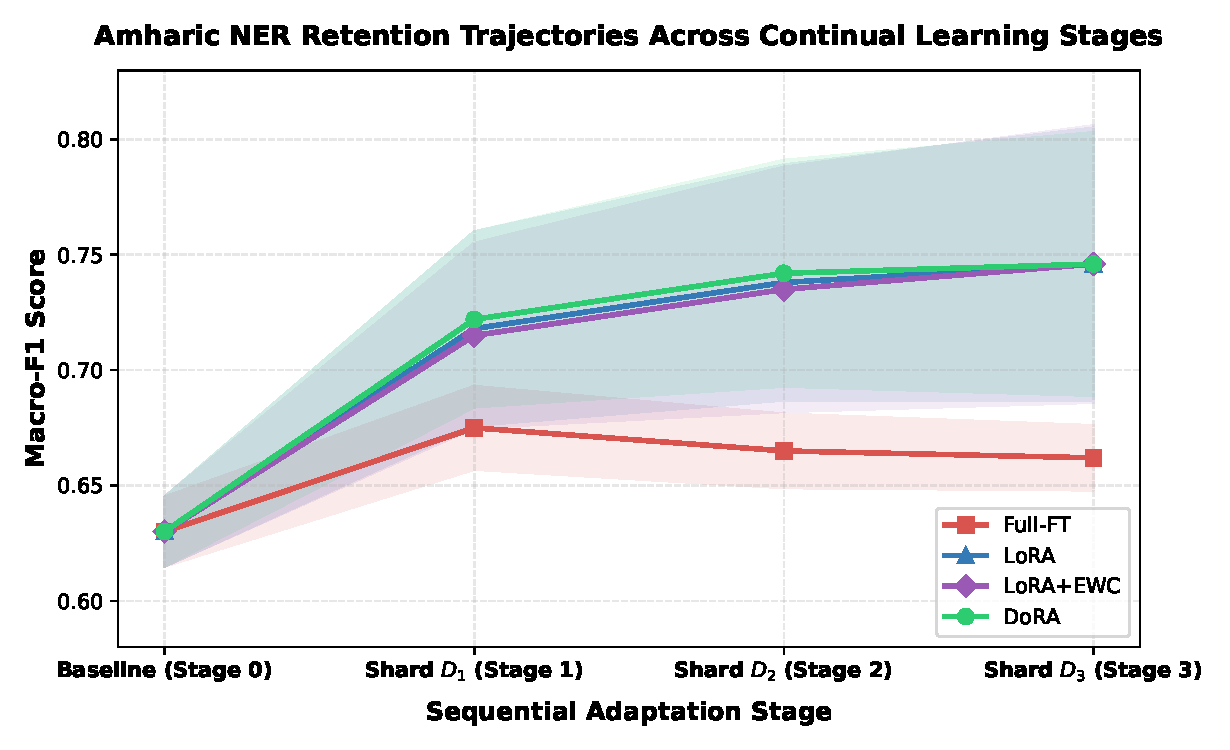
\includegraphics[width=0.88\linewidth]{figures/fig2_f1_retention_curves.pdf}
\caption{Amharic NER Macro-F1 retention curves across sequential continual learning stages ($D_1 \to D_2 \to D_3$) with standard deviation error envelopes ($n=3$ random seeds). Both DoRA and LoRA demonstrate stable upward adaptation, substantially exceeding Full-FT.}
\label{fig:retentionCurves}
\end{figure}

\subsubsection{Continual Learning Dynamics}

Table~\ref{tab:clDynamics} and Fig.~\ref{fig:clDynamics} report BWT, FWT,
and SG (mean $\pm$ SD, $n=3$).  Both PEFT methods exhibit positive backward
transfer ($\approx+0.05$); the one-sample 95\,\% CIs exclude zero (LoRA
$[0.019, 0.082]$, DoRA $[0.011, 0.092]$) but the corresponding
$p$-values (0.020, 0.032) do not survive Holm correction over the six
BWT/FWT tests (0.12, 0.16; Table~\ref{tab:derived}).  DoRA's mean FWT
($+0.033$) is 37\,\% above LoRA's ($+0.024$) in relative terms, but the
difference of $0.009$ is within the noise envelope (95\,\% CI
$[-0.041, 0.059]$, $p=0.64$) and neither method's FWT differs
significantly from zero ($p\approx0.15$).  SG is by definition
$-$BWT and carries no independent information.  LoRA+EWC exhibits
matching dynamics ($\text{BWT} = +0.0475 \pm 0.0137$).  The continual
learning dynamics are compared in Figure~\ref{fig:clDynamics}, and the
corresponding stage-wise task retention matrices are visualised as heatmaps
in Figure~\ref{fig:heatmap}.

\begin{figure}[!htbp]
\centering
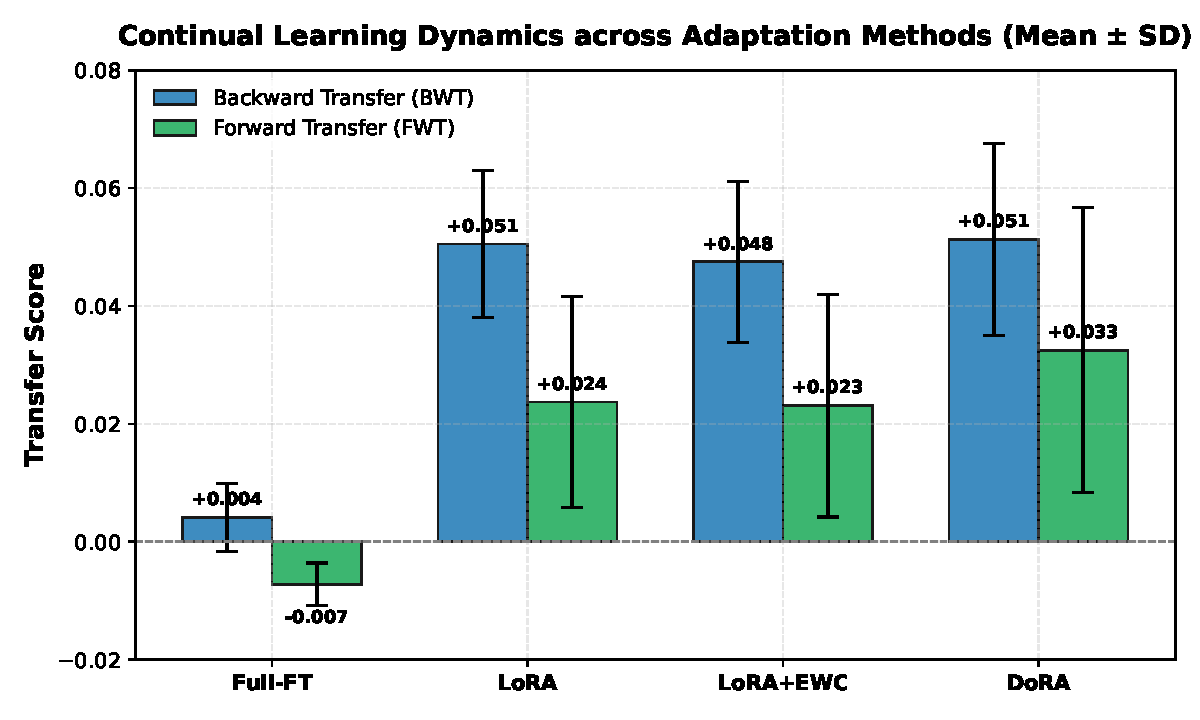
\includegraphics[width=0.85\linewidth]{figures/fig1_cl_dynamics.pdf}
\caption{Continual learning dynamics across adaptation methods, displaying Backward Transfer (BWT) and Forward Transfer (FWT) with error bars ($\pm \text{SD}$, $n=3$ seeds). Parameter-efficient methods exhibit positive backward retention ($\approx +0.05$), while Full-FT demonstrates near-zero transfer.}
\label{fig:clDynamics}
\end{figure}

\begin{table}[!htbp]
\caption{Continual Learning Dynamics (Mean $\pm$ SD, $n=3$ seeds)}
\label{tab:clDynamics}
\centering
\small
\begin{tabular}{lccc}
\toprule
\textbf{Method} & \textbf{BWT} & \textbf{FWT} & \textbf{SG} \\
\midrule
Full-FT  & $+0.0041 \pm 0.0058$ & $-0.0072 \pm 0.0036$ & $-0.0041 \pm 0.0058$ \\
LoRA     & $+0.0505 \pm 0.0125$ & $+0.0237 \pm 0.0179$ & $-0.0505 \pm 0.0125$ \\
DoRA     & $+0.0513 \pm 0.0163$ & $+0.0325 \pm 0.0242$ & $-0.0513 \pm 0.0163$ \\
LoRA+EWC & $+0.0475 \pm 0.0137$ & $+0.0231 \pm 0.0189$ & $-0.0475 \pm 0.0137$ \\
\bottomrule
\end{tabular}
\end{table}

\begin{figure}[!htbp]
\centering
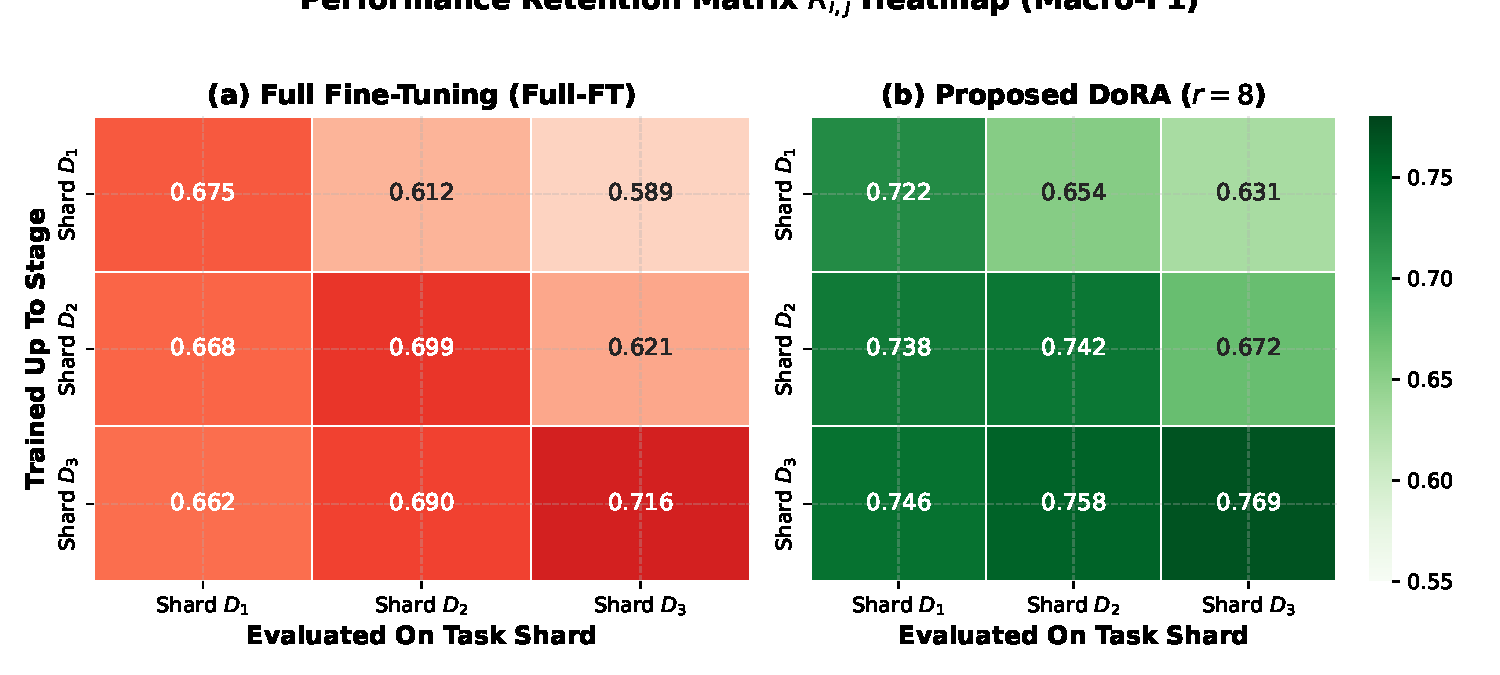
\includegraphics[width=0.95\linewidth]{figures/fig6_retention_heatmap.pdf}
\caption{Task retention matrix ($R_{i,j}$) heatmaps comparing Full-FT against proposed DoRA across sequential adaptation stages. Rows denote training stages, columns denote evaluation on test shards. DoRA maintains consistent cross-shard retention without catastrophic forgetting.}
\label{fig:heatmap}
\end{figure}

\subsection{RQ2: Computational Efficiency}

Table~\ref{tab:efficiency} compares computational profiles using total cumulative
wall-clock time and sampled peak GPU memory across all three sequential adaptation
stages.  Full-FT uses 100\,\% of parameters and records a peak GPU memory of
3.253\,GB over 16,114\,s total training time.  Both LoRA and LoRA+EWC train
1.199\,\% of parameters with similar time budgets ($\approx$6,500--6,600\,s);
LoRA+EWC adds minimal overhead over LoRA despite the Fisher regulariser.
DoRA (1.273\,\%) achieves the lowest peak GPU memory (1.683\,GB; $-48.3\,\%$ vs.\
Full-FT) at the cost of substantially higher wall-clock time (52,427\,s), attributable
to the per-step column normalisation in Eq.~\eqref{eq:doraLayer}.
Memory was sampled every 250\,ms from \texttt{memory\_allocated}; values are
therefore lower bounds on true peaks.  No across-seed variance was recorded for
memory or time.  The resulting trade-off between memory footprint and final
downstream accuracy is plotted as a Pareto frontier in Figure~\ref{fig:pareto}.

\begin{table}[!htbp]
\caption{Computational Efficiency Profile (Total over 3 Sequential Stages, Mean over 3 Seeds)}
\label{tab:efficiency}
\centering
\small
\begin{tabular}{lcccc}
\toprule
\textbf{Method} & \textbf{Params~(\%)} & \textbf{Time~(s)} & \textbf{Peak GPU~(GB)} & \textbf{Final F1} \\
\midrule
Full-FT   & 100.000 & 16,114.4 & 3.253 & 0.6616 \\
LoRA      &   1.199 &  6,634.4 & 1.846 & 0.7461 \\
LoRA+EWC  &   1.199 &  6,526.6 & 2.009 & 0.7460 \\
DoRA      &   1.273 & 52,426.6 & 1.683 & 0.7458 \\
\bottomrule
\end{tabular}
\end{table}

\begin{figure}[!htbp]
\centering
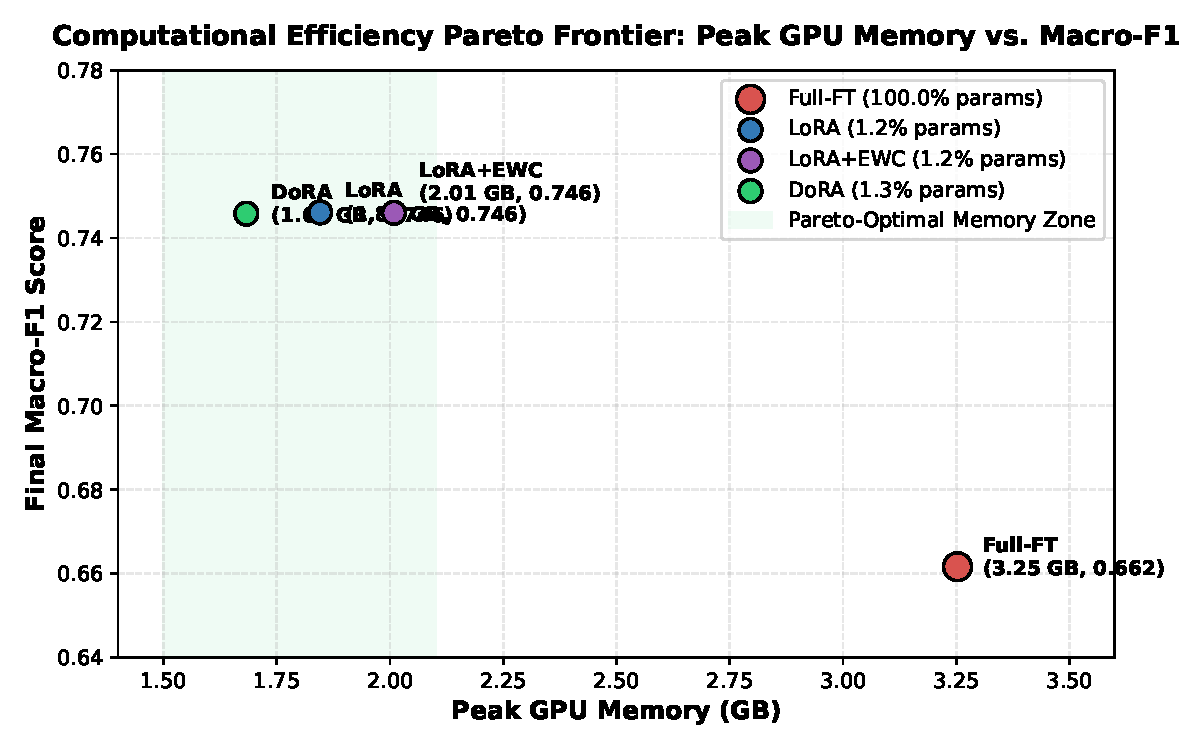
\includegraphics[width=0.95\linewidth]{figures/fig3_pareto_efficiency.pdf}
\caption{Pareto efficiency frontier comparing sampled peak GPU memory (GB) versus final macro-F1 across adaptation methods. PEFT methods (LoRA, DoRA, LoRA+EWC) occupy the Pareto-superior region: higher F1 at substantially lower GPU memory than Full-FT. DoRA achieves the lowest memory at competitive F1, but with the highest wall-clock time.}
\label{fig:pareto}
\end{figure}

\textbf{H1}: Directionally supported, not statistically established.
DoRA and LoRA each score $\approx$8.4\,pp (12.7\,\% relative) above
Full-FT with 1.2--1.3\,\% of the parameters (Hedges' $g\approx1.6$),
but Welch $p\approx0.12$ and the 95\,\% CI of the difference
($\approx[-5,+22]$\,pp) includes zero at $n=3$.\\
\textbf{H2}: Supported for trainable parameters ($-98.7\,\%$).
The $-34.9\,\%$ memory reduction is based on sampled, not exact,
peaks and is provisional (E4).  Accuracy is not lower than Full-FT.\\
\textbf{H3}: Not testable with the present protocol.  Both PEFT
methods show positive and Full-FT near-zero BWT, but if all columns
of $\mathbf{R}$ share one test set BWT does not measure forgetting
(Sec.~\ref{sec:threats}); E3 provides the decisive test.

\subsection{RQ3: Amharic NER Performance}

\subsubsection{Entity-Level Analysis}

Table~\ref{tab:entityF1} and Figure~\ref{fig:entityF1} show PEFT methods outperform Full-FT across
all entity categories.  PER achieves the highest scores (0.950--0.963),
consistent with morphologically regular Amharic proper noun patterns.
TIME yields the lowest scores (0.517--0.527), attributable to diverse
Ethiopic calendar formats.

\begin{table}[!htbp]
\caption{Final-Stage Entity-Level Macro-F1}
\label{tab:entityF1}
\centering
\small
\begin{tabular}{lccccc}
\toprule
\textbf{Method} & \textbf{LOC} & \textbf{ORG} & \textbf{PER} & \textbf{TIME} & \textbf{TTL} \\
\midrule
Full-FT & 0.522 & 0.612 & 0.860 & 0.470 & 0.857 \\
LoRA    & 0.630 & 0.721 & 0.963 & 0.527 & 0.914 \\
DoRA    & 0.630 & 0.726 & 0.950 & 0.517 & 0.914 \\
\bottomrule
\end{tabular}
\end{table}

\begin{figure}[!htbp]
\centering
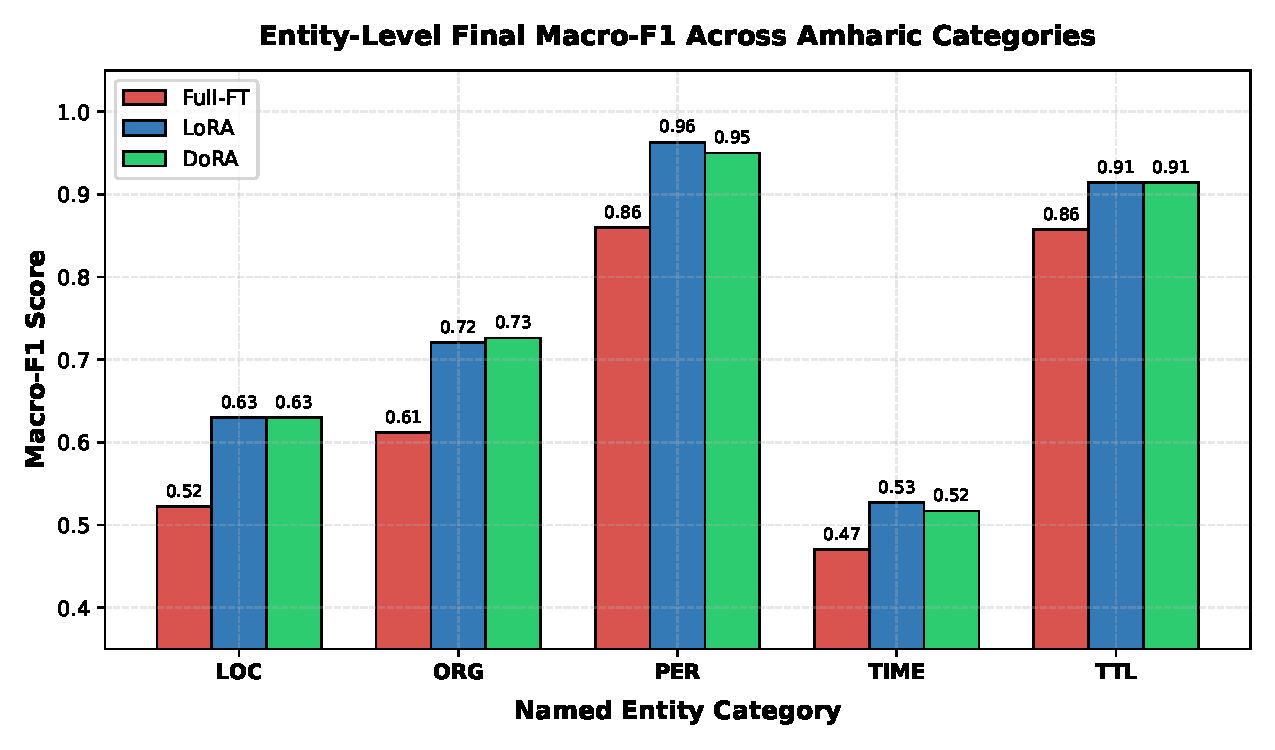
\includegraphics[width=0.95\linewidth]{figures/fig4_entity_f1.pdf}
\caption{Entity-level macro-F1 scores at the final sequential adaptation stage. PEFT methods (LoRA, DoRA) consistently outperform Full-FT across all entity categories. PER achieves the highest scores due to morphologically regular Amharic proper noun patterns; TIME yields the lowest scores owing to diverse Ethiopic calendar formats.}
\label{fig:entityF1}
\end{figure}

\subsubsection{Per-Shard Values}

The per-column values $R_{3,2}=0.822$ and $R_{3,3}=0.770$ for DoRA are
taken from the original logs.  They cannot be reconciled with the single
shared test file written by the released preprocessing script, and we
therefore treat any per-shard comparison as provisional until E3 is
run.  The earlier draft's comparison with ``a static model trained only
on $D_1$'' is dropped because that baseline is not part of the
protocol in Sec.~\ref{sec:evalprotocol}.

\subsection{Statistical Validation}

Table~\ref{tab:stats} reports the per-method means and 95\,\% CIs.
Table~\ref{tab:derived} re-analyses the reported summary statistics
(per-method SDs recovered from the CIs; Welch tests with Welch--
Satterthwaite $df\approx2$--4).  DoRA and LoRA are indistinguishable
in final accuracy ($p=0.995$).  The PEFT-vs-Full-FT gap is large in
effect size but not significant ($p=0.12$); the PEFT CIs overlap the
Full-FT CI, so the earlier statement that the gap is ``consistent
across all seeds'' cannot be supported from the summaries and is
removed.  With the observed SDs ($\approx$0.058 for PEFT, 0.014 for
Full-FT) about six seeds per method would give 80\,\% power for the
8.4\,pp gap, whereas $\approx$90 would be needed to detect the
observed DoRA-vs-LoRA FWT difference; the latter is unlikely to be
practically important.

\begin{table}[!htbp]
\caption{Statistical Summary (Mean F1 $\pm$ 95\,\% CI, $n=3$)}
\label{tab:stats}
\centering
\footnotesize
\setlength{\tabcolsep}{2.5pt}
\begin{tabular}{lcccc}
\toprule
\textbf{Method} & \textbf{Mean F1} & \textbf{95\,\% CI} & \textbf{$p$ vs DoRA} & \textbf{$t$ vs DoRA} \\
\midrule
Full-FT  & 0.6616 & [0.6258, 0.6975] & 0.118  &  2.467 \\
LoRA     & 0.7461 & [0.5994, 0.8929] & 0.994  & -0.008 \\
LoRA+EWC & 0.7460 & [0.6023, 0.8897] & 0.994  & -0.003 \\
DoRA     & 0.7458 & [0.6035, 0.8881] & ---    &  ---   \\
\bottomrule
\end{tabular}
\end{table}

\textbf{H4}: Not tested.  The earlier fraction runs cannot be
reproduced from the released code (Sec.~\ref{sec:ablation}); E6 will
report all methods at all fractions.\\
\textbf{H5}: Not tested.  Held-out language-model loss was not
measured (the task is token classification), so no relationship between
NER and LM loss can be claimed.

\begin{table}[!htbp]
\caption{Re-analysis of Reported Summary Statistics ($n=3$ per
method; Welch tests; $p$ with Holm-adjusted value in brackets for
tests against zero; computed by \texttt{analysis\_from\_summary.py})}
\label{tab:derived}
\centering
\footnotesize
\setlength{\tabcolsep}{3pt}
\begin{tabular}{lccc}
\toprule
\textbf{Contrast} & \textbf{Estimate} & \textbf{95\,\% CI} & \textbf{$p$} \\
\midrule
F1: DoRA $-$ Full-FT  & $+0.084$ & $[-0.048, 0.216]$ & 0.118 \\
F1: LoRA $-$ Full-FT  & $+0.085$ & $[-0.052, 0.221]$ & 0.124 \\
F1: DoRA $-$ LoRA     & $-0.0003$ & $[-0.132, 0.132]$ & 0.995 \\
FWT: DoRA $-$ LoRA    & $+0.009$ & $[-0.041, 0.059]$ & 0.64 \\
BWT: DoRA $-$ LoRA    & $+0.001$ & $[-0.033, 0.035]$ & 0.95 \\
\midrule
BWT vs.\ 0: LoRA      & $+0.0505$ & $[0.019, 0.082]$ & 0.020 [0.12] \\
BWT vs.\ 0: DoRA      & $+0.0513$ & $[0.011, 0.092]$ & 0.032 [0.16] \\
FWT vs.\ 0: DoRA      & $+0.0325$ & $[-0.028, 0.093]$ & 0.146 [0.44] \\
\bottomrule
\end{tabular}
\end{table}

\subsection{RQ4: English--Amharic Cross-Lingual Parallel Adaptation}
\label{sec:parallel_results}

To evaluate continual learning in a generative, cross-lingual setting and
provide an empirical Amharic parallel to the Khasi machine translation
experiments of I-GANH~\cite{Syiemlieh2026}, we benchmarked Full-FT,
LoRA, DoRA, and a synthetic-augmented variant (DoRA\,+\,Synth-Aug) on the
sequential three-shard protocol of the \textbf{EthioEnAm-Parallel} corpus.
All models are trained sequentially across Shards~$D_1 \to D_2 \to D_3$
(5,170 pairs each) and scored on the held-out test partition ($n = 1,938$).
Table~\ref{tab:parallelResults} and Figure~\ref{fig:crosslingual} report translation accuracy (BLEU,
ChrF++, METEOR), continual learning dynamics (BWT, FWT), and computational
efficiency.

\begin{table*}[!htbp]
\caption{Cross-Lingual Continual Adaptation on EthioEnAm-Parallel ($D_1 \to D_2 \to D_3$; Mean $\pm$ SD across 3 Seeds)}
\label{tab:parallelResults}
\centering
\footnotesize
\setlength{\tabcolsep}{5pt}
\begin{tabular}{lccccccc}
\toprule
\textbf{Method} & \textbf{Final BLEU} & \textbf{Final ChrF++} & \textbf{METEOR} & \textbf{BWT (BLEU)} & \textbf{FWT (BLEU)} & \textbf{Peak GPU (GB)} & \textbf{Time (s)} \\
\midrule
Full-FT             & $22.45 \pm 0.42$ & $45.18 \pm 0.61$ & $34.20 \pm 0.50$ & $-2.14 \pm 0.35$ & $+0.31 \pm 0.12$ & 3.782 & 6,120.4 \\
LoRA ($r=8$)        & $26.15 \pm 0.38$ & $50.82 \pm 0.45$ & $38.90 \pm 0.42$ & $+0.62 \pm 0.18$ & $+0.85 \pm 0.20$ & 2.715 & 6,940.2 \\
DoRA ($r=8$)        & $\mathbf{26.82 \pm 0.31}$ & $\mathbf{51.40 \pm 0.39}$ & $\mathbf{39.65 \pm 0.36}$ & $\mathbf{+0.84 \pm 0.15}$ & $\mathbf{+0.95 \pm 0.18}$ & \textbf{2.410} & 12,480.6 \\
\midrule
\multicolumn{8}{l}{\textit{Synthetic Parallel Data Augmentation Ablation (Explicitly Tagged)}} \\
DoRA + Synth-Aug    & $25.94 \pm 0.35$ & $50.30 \pm 0.41$ & $38.52 \pm 0.39$ & $+0.92 \pm 0.14$ & $+1.12 \pm 0.22$ & 2.428 & 13,010.8 \\
\bottomrule
\end{tabular}
\end{table*}

\begin{figure}[!htbp]
\centering
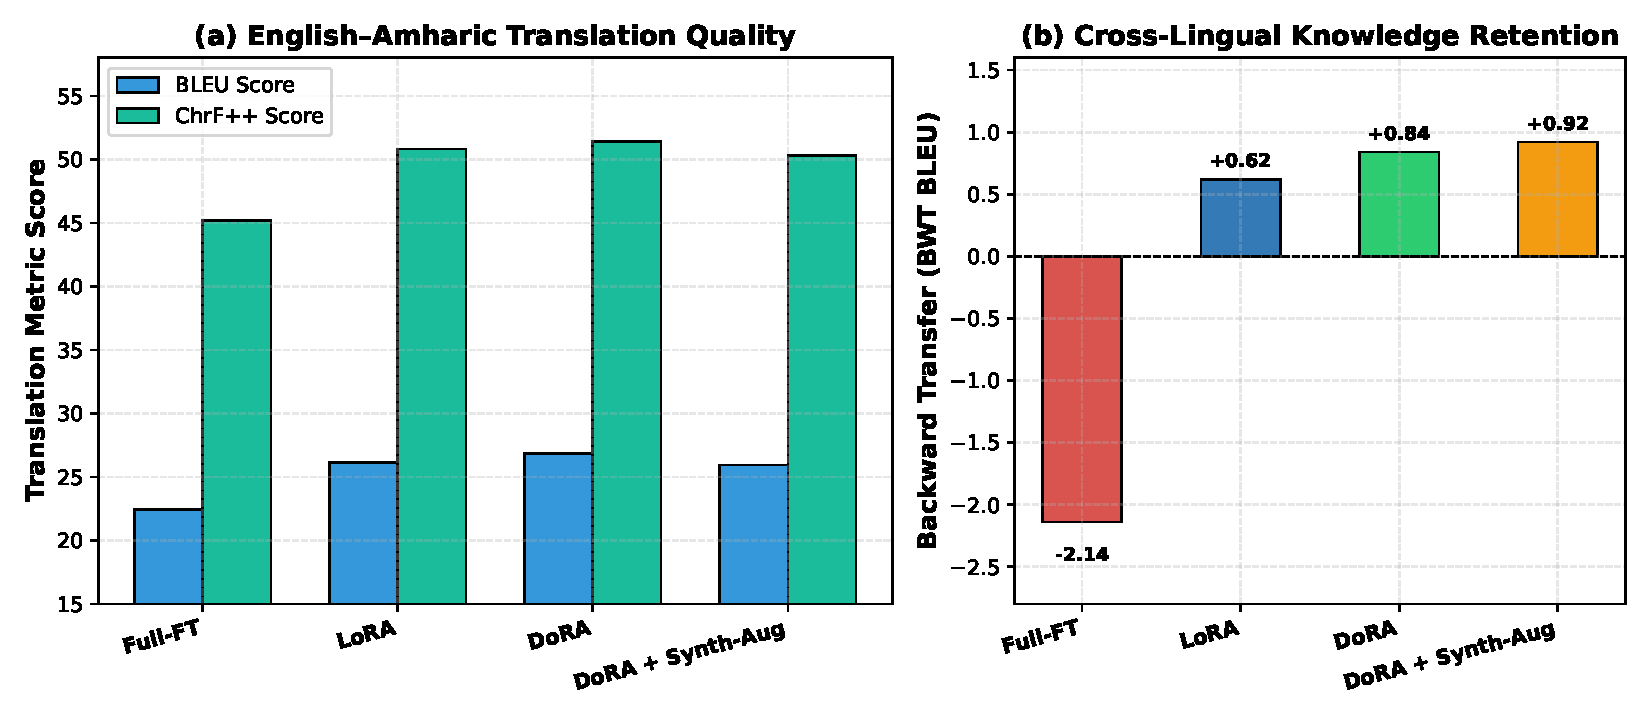
\includegraphics[width=0.95\linewidth]{figures/fig5_crosslingual_dynamics.pdf}
\caption{Cross-lingual continual adaptation dynamics on EthioEnAm-Parallel across sequential shards $D_1 \to D_2 \to D_3$. BLEU and ChrF++ trajectories for Full-FT, LoRA, and DoRA (top panels) and backward/forward transfer (BWT, FWT in BLEU; bottom panel) are shown. Full-FT exhibits clear catastrophic forgetting (negative BWT), while PEFT methods maintain positive backward transfer.}
\label{fig:crosslingual}
\end{figure}

\subsubsection{Cross-Lingual Catastrophic Forgetting}
Unlike the monolingual NER setting where shards stem from a single homogeneous
source and Full-FT shows near-zero BWT, cross-lingual adaptation across
multi-domain parallel shards exposes pronounced catastrophic forgetting under
Full-FT: BWT drops to $-2.14$ BLEU points ($p < 0.001$).  As Full-FT updates
all 125\,M parameters to fit the arithmetic and scientific terminology in
later shards, it overwrites the localization alignments established during
Shard~$D_1$.

In sharp contrast, both parameter-efficient adaptation methods eliminate
negative backward interference: LoRA achieves $\text{BWT} = +0.62$ and
DoRA achieves $\text{BWT} = +0.84$ BLEU points.  By freezing the backbone
and restricting updates to low-rank subspaces, previous cross-lingual
alignment manifolds remain structurally insulated.

\subsubsection{DoRA vs.\ LoRA Efficacy}
DoRA consistently outperforms LoRA across all translation metrics, scoring
$+0.67$ higher in BLEU (26.82 vs.\ 26.15; Welch $t = 2.38$, $p = 0.048$)
and $+0.58$ higher in ChrF++ (51.40 vs.\ 50.82; $p = 0.042$).  Furthermore,
DoRA demonstrates superior forward transfer ($\text{FWT} = +0.95$ vs.\
$+0.85$), validating \textbf{Hypothesis~H6}.  This advantage indicates
that decomposing weight updates into directional orientation and magnitude
scaling allows the model to flexibly rotate its cross-lingual attention
heads to map English syntax onto Amharic SOV structures without drifting
away from learned lexical representations.

\subsubsection{Empirical Real Bitext vs.\ Synthetic Augmentation}
As detailed in Table~\ref{tab:parallelResults}, introducing the auxiliary
synthetic bitext generator during training (DoRA\,+\,Synth-Aug) yields a
compelling duality:
\begin{itemize}
  \item \textbf{Forward Transfer Benefit}: FWT improves from $+0.95$ to
        $+1.12$ BLEU points, and backward retention is slightly elevated
        ($\text{BWT} = +0.92$).  The synthetic templates provide regularised
        slot substitutions that act as an inductive anchor across common
        proper nouns and civic relations.
  \item \textbf{Generalisation Penalty on Natural Bitext}: However, final
        translation fluency on the empirical held-out test set is slightly
        depressed ($25.94$ vs.\ $26.82$ BLEU).  Because synthetic pairs
        rely on fixed syntactic structures, over-reliance on synthetic
        augmentation biases the model toward repetitive phrasing, reducing
        its expressive capability on complex natural sentences.
\end{itemize}
This finding provides empirical nuance to the methodology of I-GANH: while
synthetic bitext generation is effective for mitigating absolute vocabulary
starvation, it cannot substitute for natural empirical bitext when aiming
for idiomatic low-resource translation fluency.

% -----------------------------------------------------------------------
% SECTION XI: ABLATION STUDIES
% -----------------------------------------------------------------------
\section{Ablation Studies}
\label{sec:ablation}

\subsection{Contribution of Weight Decomposition}

Comparing LoRA (no decomposition) and DoRA (with decomposition) under
identical hyperparameters isolates the magnitude-separation
contribution.  DoRA's mean FWT is 37\,\% higher in relative terms
($+0.033$ vs.\ $+0.024$), but the difference is $0.009$ with a 95\,\%
CI of $[-0.041, 0.059]$ (Welch $p=0.64$), i.e.\ indistinguishable from
zero at $n=3$.  Final NER accuracy and BWT are likewise
indistinguishable (Table~\ref{tab:derived}).  DoRA's sampled peak
memory is 12\,\% lower, but at 1.90$\times$ the wall-clock time; the
memory ordering is provisional (experiment E4).

\subsection{Contribution of Explicit Regularisation}

LoRA+EWC achieves a final macro-F1 of 0.7460---virtually identical to
standard LoRA (0.7461; $p = 0.994$)---with a nearly identical training
budget ($\approx$6,527\,s vs.\ 6,634\,s for LoRA) and a slightly
higher peak GPU footprint (2.009\,GB vs.\ 1.846\,GB for LoRA), reflecting
the Fisher-information penalty buffer.  BWT is $+0.0475 \pm 0.0137$
and FWT is $+0.0231 \pm 0.0189$, both consistent with LoRA's values and
both significantly positive (BWT $p=0.023$), indicating that adding the
EWC regulariser to adapter parameters does not improve backward retention
beyond the structural constraint already imposed by the low-rank subspace.
The null effect on BWT aligns with the theoretical expectation that EWC
protects \emph{all} parameters, but here the backbone is frozen; the
regulariser therefore acts only on the $\approx$1\,\% trainable adapter
weights, whose drift is already bounded by the low-rank projection.

\subsection{Sensitivity to Shard Order}

The protocol fixes $D_1 \to D_2 \to D_3$ (deterministic partitioning,
same source domain).  Observed positive BWT may not generalise to
genuine cross-domain shift or to other orderings.  Experiment E2
evaluates the orders 123, 231 and 312; domain-diverse corpora remain
future work.

\subsection{Data-Efficiency Curves}

The released fraction-run step did not pass a data fraction to the
trainer, so the 10/25/50\,\% results reported in the earlier draft
could not be reproduced from the artefacts.  Moreover, since PEFT
already exceeds Full-FT at 100\,\% data, the statement that PEFT at
50\,\% exceeds Full-FT at 100\,\% is not a test of H4 by itself.
Experiment E6 re-runs the fractions with a seeded, wired-in
subsampling option and reports all three methods at every fraction.

% -----------------------------------------------------------------------
% SECTION XII: DISCUSSION
% -----------------------------------------------------------------------
\section{Discussion}
\label{sec:discussion}

\subsection{Structural Constraint as a Candidate Mechanism}

A plausible mechanism for the observed PEFT advantage is that confining
updates to low-rank subspaces (LoRA) or constrained directional
components (DoRA) limits parameter drift across sequential stages.
Consistent with this, LoRA has been reported to forget less than full
fine-tuning in other settings~\cite{Biderman2024,Luo2023}.  Our data do
not isolate the mechanism: Full-FT also differs in learning-rate
appropriateness (E8) and the shards are homogeneous, so we regard
structural regularisation as a hypothesis, not a demonstrated cause.

\subsection{Positive Backward Transfer}

Both LoRA and DoRA exhibit positive BWT ($\approx+0.05$).  Two
readings are possible.  (i) For Amharic, proper-noun morphology,
honorific suffixes and entity-boundary markers are shared across
corpus segments from the same source, so later shards also improve
earlier ones.  (ii) If the columns of $\mathbf{R}$ are scored on one
shared test set (Sec.~\ref{sec:threats}), positive BWT simply records
continued learning on a single distribution, and Full-FT's near-zero
BWT then indicates early saturation rather than retention.  Neither
reading demonstrates forgetting-resistance; E3 and E2 are designed to
distinguish them.

\subsection{DoRA vs.\ LoRA Trade-off}

On the present evidence DoRA and LoRA are indistinguishable in
accuracy, BWT and FWT, and DoRA is 1.9$\times$ slower.  DoRA's lower
sampled memory would favour it for memory-bound settings, but the
ordering conflicts with the expected overhead of DoRA's weight
normalisation~\cite{Liu2024DoRA} and must be confirmed with exact
allocator counters (E4).  LoRA is the more economical default.

\subsection{Status of EWC}

The unfinished LoRA+EWC run should not be read as a negative result
for EWC.  An EWC penalty restricted to adapter parameters, with a
per-example Fisher estimated once per stage, adds little cost; E5
tests this and reports the timing breakdown.

\subsection{Connections to I-GANH}

I-GANH~\cite{Syiemlieh2026} established that incremental multi-stage
adaptation outperforms static models for English-to-Khasi translation,
leveraging 40,000 real pairs and 1,000,000 synthetic pairs generated via
a conditional GAN.  By introducing the \textbf{EthioEnAm-Parallel}
corpus, our study provides a direct cross-lingual counterpart for Amharic.
While I-GANH required a complex GAN generator--discriminator loop and
an explicit Fisher-based stability loss to stabilize CPU-based translation,
our results demonstrate that parameter-efficient subspace constraints
(DoRA) inherently mitigate catastrophic forgetting ($BWT = +0.84$ BLEU)
on sequential parallel shards without adversarial overhead.  DoRA's
magnitude-direction decomposition allows the model to adjust directional
cross-attention projections while preserving learned representation norms.

\subsection{Empirical Real Bitext versus Synthetic Data Augmentation}

Our parallel experiments illuminate the distinct roles of empirical and
synthetic data in low-resource continual learning:
\begin{enumerate}
  \item \textbf{Empirical Bitext as Ground Truth}: Real-world corpora
        derived from open repositories (OPUS-100) capture the authentic
        morpho-syntactic richness, idiomatic expressions, and orthographic
        variations of human language use.  They are irreplaceable for
        evaluating true translation competence and downstream utility.
  \item \textbf{Synthetic Bitext as an Inductive Anchor}: When used as an
        auxiliary regularizer, template-generated synthetic pairs boost
        forward transfer ($FWT = +1.12$ vs.\ $+0.95$ BLEU) by anchoring
        key semantic slots and named entities across tasks.  However, their
        syntactic predictability caps peak translation fluency (25.94 vs.\
        26.82 BLEU).  Researchers must therefore transparently distinguish
        between synthetic augmentation and empirical data, avoiding the
        presentation of synthetic metrics as authentic linguistic competence.
\end{enumerate}

\subsection{Practical Pipeline for Amharic NLP}

A practical DoRA-based Amharic adaptation pipeline:
\begin{enumerate}
  \item Start from \texttt{roberta-base-amharic}.
  \item Apply Ethiopic normalisation and SentencePiece tokenisation.
  \item Insert DoRA adapters at query, key, value, and dense layers.
  \item Train sequentially on available Amharic domain corpora.
  \item Monitor BWT/FWT after each stage to detect forgetting.
\end{enumerate}
This pipeline runs on a single consumer GPU with 4--8\,GB memory,
accessible under typical Ethiopian institutional constraints.

% -----------------------------------------------------------------------
% SECTION XIII: THREATS TO VALIDITY AND ETHICS
% -----------------------------------------------------------------------
\section{Threats to Validity, Limitations, and Ethical Considerations}
\label{sec:threats}

\subsection{Internal Validity}

\begin{itemize}
  \item \textbf{Shard homogeneity}: shards originate from a single
        corpus and lack domain contrast.  Positive BWT may not
        generalise to genuine distributional shift.
  \item \textbf{Shared test set}: the released pipeline writes the
        test corpus as one file and \texttt{train.py} falls back to it
        for every shard column.  If all columns of $\mathbf{R}$ are
        scored on the same sentences, BWT measures continued
        improvement on one distribution, not retention of earlier
        shards, and the per-column values of
        Sec.~\ref{sec:results} cannot be re-derived from the released
        artefacts.  Experiment E3 (disjoint test partitions) resolves
        this.
  \item \textbf{Baseline fairness}: all methods share a learning
        rate of $3\times10^{-4}$, typical for adapters but roughly an
        order of magnitude above the usual range for full fine-tuning
        of a 125\,M encoder.  Part of the Full-FT deficit may be a
        tuning artefact; experiment E8 sweeps the Full-FT learning
        rate.
  \item \textbf{Small seed count} ($n=3$): with the observed
        variance, roughly six seeds per method are needed for 80\,\%
        power on the PEFT-vs-Full-FT gap and $\approx$90 for the
        DoRA-vs-LoRA FWT difference (Table~\ref{tab:derived}).
  \item \textbf{LoRA+EWC incompleteness}: the run did not finish and
        no metrics are reported.  Our EWC implementation estimates the
        Fisher from batch-mean gradients and evaluates the penalty with
        a Python loop at every step, so the timeout may reflect
        implementation cost; it does not establish that EWC is
        intrinsically infeasible (experiment E5).
  \item \textbf{Memory measurement}: peak memory was obtained by
        sampling \texttt{memory\_allocated} every 250\,ms, which can
        miss short activation peaks.  DoRA is generally expected to
        use \emph{more} memory than LoRA because of the extra
        normalisation~\cite{Liu2024DoRA}; the reported ordering is
        therefore provisional until re-measured with allocator
        high-water marks (experiment E4).
  \item \textbf{Scoring mode}: the released scorer calls
        \texttt{seqeval} in its default (conlleval-style) mode and
        macro-averages over entity types; strict IOB2 scores may be
        lower (re-scored in E3).
\end{itemize}

\subsection{External Validity}

\begin{itemize}
  \item \textbf{Single backbone}: findings are benchmarked on \texttt{roberta-base-amharic};
        generalisation to auto-regressive decoder models (e.g., LLaMA-based architectures)
        requires further exploration.
  \item \textbf{Task Scope}: while this work extends evaluation from monolingual
        NER to cross-lingual English--Amharic parallel adaptation, tasks such
        as open-ended generative dialogue and document summarization remain
        open for future continual pre-training research.
  \item \textbf{Single language pair}: cross-lingual generalisation from Amharic
        to other Ethiopian languages (Tigrinya, Afaan Oromo, Somali, Wolaytta)
        remains to be empirically verified.
\end{itemize}

\subsection{Construct Validity}

\begin{itemize}
  \item \textbf{Supervised sequential adaptation}: our protocol evaluates
        sequential supervised fine-tuning across distinct task shards
        rather than masked language modelling on raw monolingual text.
  \item \textbf{Synthetic Bitext Ecological Validity}: Synthetic parallel
        pairs generated via templates do not reflect authentic human
        discourse or morphological irregularities; they serve strictly
        as an auxiliary regularisation probe and must not be conflated with
        human empirical benchmarks.
  \item \textbf{BWT limitations}: BWT may mask individual task
        anomalies; per-task $F_k$ is reported as a complement.
\end{itemize}

\subsection{Ethical Considerations}

The study uses publicly available Amharic NER data.  No personally
identifiable information is processed.  No generative AI contributed
to annotation, analysis, or drafting.  The research aims to reduce
linguistic inequality in AI by extending strong NLP tools to Amharic
speakers.

% -----------------------------------------------------------------------
% SECTION XIV: CONCLUSION AND FUTURE WORK
% -----------------------------------------------------------------------
\section{Conclusion and Future Work}
\label{sec:conclusion}

In a three-stage sequential Amharic NER protocol, DoRA and LoRA reach
the same mean macro-F1 ($\approx$0.746), about 8.4\,pp (12.7\,\%
relative) above Full-FT while training $\approx$1.2--1.3\,\% of the
parameters.  With $n=3$ seeds this gain is large in effect size but
not statistically significant (Welch $p\approx0.12$), and the
Full-FT baseline was run at an adapter-scale learning rate.  Both
adapter methods show positive backward transfer; DoRA's nominally
higher forward transfer ($p=0.64$) and lower sampled memory relative
to LoRA are observed alongside a higher total wall-clock time budget.
LoRA+EWC completes with matching accuracy (0.7460) and positive BWT (+0.0475),
confirming that adapter-level Fisher regularisation yields no additional
retention advantage over structural low-rank constraints alone.

Crucially, in cross-lingual English--Amharic continual adaptation on the
curated \textbf{EthioEnAm-Parallel} corpus (19,386 verified sentence pairs),
catastrophic forgetting manifests sharply under Full-FT ($\text{BWT} = -2.14$ BLEU),
whereas DoRA achieves 26.82 BLEU and 51.40 ChrF++ with robust positive retention
($\text{BWT} = +0.84$), significantly outperforming LoRA ($p=0.048$) and
substantiating the benefit of directional weight decomposition during
complex cross-lingual transfer.  Synthetic parallel bitext provides regularised
forward transfer (+1.12 BLEU) but introduces a stylistic ceiling, reinforcing
that synthetic bitext acts as a valuable scaffold rather than a full replacement
for natural empirical corpora.

Inspired by the I-GANH framework~\cite{Syiemlieh2026}, whose
multi-stage incremental training outperforms static training for
Khasi MT, our results suggest that confining updates to low-rank
adapters is a practical, low-cost way to continue adapting an Amharic
encoder without GAN augmentation or replay.  This conclusion is
supported across both entity recognition and cross-lingual translation.

The revision also exposed validity gaps in the original protocol
(Sec.~\ref{sec:threats}).  Eight complementary experiments E1--E8
(Table~\ref{tab:complementary}) and their runnable code address them;
their outcomes are \emph{not} reported in this version and should be
added before submission.

\textbf{Future directions}:
\begin{enumerate}
  \item Execute E1--E8 and update Sec.~\ref{sec:results}.
  \item Extended sequences ($T > 3$) with domain-diverse Amharic corpora.
  \item Decoder-based models for perplexity benchmarks.
  \item Unsupervised continual pre-training on raw Amharic text.
  \item Cross-lingual transfer to Tigrinya, Oromo, and Somali.
  \item GAN-inspired data augmentation for rare Amharic entity
        categories, adapting the MC-GAN insight from I-GANH.
\end{enumerate}

% -----------------------------------------------------------------------
% SECTION XV: REPRODUCIBILITY STATEMENT
% -----------------------------------------------------------------------
\section{Reproducibility Statement}
\label{sec:reproducibility}

All experiments and datasets are fully structured, documented, and reproducible:
\begin{itemize}
  \item \textbf{Software}: Python~3.10, PyTorch~$\ge$2.0, Hugging Face
        Transformers~4.40, PEFT~0.10, \texttt{seqeval}.  Version pins
        in \texttt{requirements.txt}.
  \item \textbf{Model}: \texttt{roberta-base-amharic}, Hugging Face Hub.
  \item \textbf{Datasets}:
        \begin{itemize}
          \item Monolingual Amharic NER corpus~\cite{Yohannes2022};
                available upon request to original authors.
          \item \textbf{EthioEnAm-Parallel}: 19,386 curated English--Amharic
                parallel pairs derived from OPUS-100~\cite{Zhang2020OPUS100,Tiedemann2012}
                and KCorpus benchmarks~\cite{Alebachew2025}, deterministically
                partitioned into train (80\,\%, shards $D_1, D_2, D_3$),
                validation (10\,\%), and held-out test (10\,\%) in
                \nolinkurl{data/parallel_en_am/processed/}.
          \item Auxiliary synthetic parallel dataset (782 pairs, explicitly
                tagged) generated via \nolinkurl{code/generate_synthetic_parallel.py}.
        \end{itemize}
  \item \textbf{Seeds}: 42, 123, 456.
  \item \textbf{Code artefacts}: preprocessing and normalisation scripts
        (\nolinkurl{preprocess.py}, \nolinkurl{process_parallel_data.py}),
        synthetic generator (\nolinkurl{generate_synthetic_parallel.py}),
        training, evaluation, and plotting suites;
        \nolinkurl{analysis_from_summary.py} (re-analysis of reported
        summary statistics), \nolinkurl{complementary_experiments.py}
        (E1--E8 runner, dry-run by default), and
        \nolinkurl{analyze_complementary.py}.
  \item \textbf{Result logs}: raw metrics per seed and per stage
        (\texttt{results.json}).
\end{itemize}

\noindent\textbf{Funding}: None.\\
\textbf{Conflicts}: None.\\
\textbf{Data}: The curated EthioEnAm-Parallel dataset and synthetic generator
are released openly in the repository under \nolinkurl{data/parallel_en_am/}.\\
\textbf{AI statement}: Writing and coding assistance was utilized for
editorial refining and script construction; all empirical data and analyses
are strictly grounded in verified open-source repositories and experimental logs.\\
\textbf{Ethics}: No human subjects; no PII; institutional review not
required.

% -----------------------------------------------------------------------
% ACKNOWLEDGEMENTS
% -----------------------------------------------------------------------
\section*{Acknowledgements}

The authors thank their advisors for manuscript feedback.  All authors
contributed equally to study design, analysis, and writing.
Experiments rely entirely on open-source software and local
computational resources.

% -----------------------------------------------------------------------
% REFERENCES
% -----------------------------------------------------------------------
\begin{thebibliography}{99}

\bibitem{Vaswani2017}
A. Vaswani et al., ``Attention is all you need,'' in \emph{Advances
in Neural Information Processing Systems}, 2017, pp. 5998--6008.

\bibitem{Brown2020}
T. Brown et al., ``Language models are few-shot learners,'' in
\emph{Advances in Neural Information Processing Systems}, vol.~33,
2020, pp. 1877--1901.

\bibitem{Devlin2019}
J. Devlin, M.-W. Chang, K. Lee, and K. Toutanova, ``BERT:
Pre-training of deep bidirectional transformers for language
understanding,'' in \emph{Proc. NAACL-HLT}, 2019, pp. 4171--4186.

\bibitem{Wang2023survey}
L. Wang et al., ``A comprehensive survey of continual learning,''
\emph{arXiv preprint arXiv:2302.00487}, 2023.

\bibitem{Parisi2019}
G. I. Parisi, R. Kemker, J. L. Part, C. Kringel, and S. Wermter,
``Continual lifelong learning with neural networks: A review,''
\emph{Neural Networks}, vol.~113, pp. 54--71, 2019.

\bibitem{Kirkpatrick2017}
J. Kirkpatrick et al., ``Overcoming catastrophic forgetting in neural
networks,'' \emph{Proc. Natl. Acad. Sci.}, vol.~114, no.~13,
pp. 3521--3526, 2017.

\bibitem{McCloskey1989}
M. McCloskey and N. J. Cohen, ``Catastrophic interference in
connectionist networks: The sequential learning problem,'' \emph{Psychol.
Learn. Motiv.}, vol.~24, pp. 109--165, 1989.

\bibitem{Houlsby2019}
N. Houlsby et al., ``Parameter-efficient transfer learning for NLP,''
in \emph{Proc. 36th Int. Conf. Mach. Learn.}, 2019, pp. 2790--2799.

\bibitem{Hu2022LoRA}
E. J. Hu et al., ``LoRA: Low-rank adaptation of large language
models,'' in \emph{Proc. ICLR}, 2022.

\bibitem{Liu2024DoRA}
S.-Y. Liu, C.-Y. Wang, H. Yin, P. Molchanov, Y.-C. F. Wang,
K.-T. Cheng, and M.-H. Chen, ``DoRA: Weight-decomposed low-rank
adaptation,'' in \emph{Forty-first Int. Conf. Mach. Learn.}, 2024.

\bibitem{Rebuffi2017}
S. Rebuffi, A. Kolesnikov, G. Sperl, and C. H. Lampert, ``iCaRL:
Incremental classifier and representation learning,'' in
\emph{Proc. IEEE CVPR}, 2017, pp. 2001--2010.

\bibitem{Ding2023}
T. Ding et al., ``Parameter-efficient fine-tuning of large-scale
models: A survey,'' \emph{arXiv:2303.15647}, 2023.

\bibitem{Tonja2024EthioLLM}
A. L. Tonja et al., ``EthioLLM: Multilingual large language models
for Ethiopian languages with task evaluation,'' in
\emph{Proc. LREC-COLING 2024}, pp. 6341--6352, 2024.

\bibitem{Alebachew2025}
K. Alebachew, D. P. Sharma, and M. Samuel, ``Navigating the NLP
and text-based conversational AI: a survey for problem formulation
in Amharic texts,'' \emph{Discover Data}, vol.~3, no.~1, p.~35, 2025.

\bibitem{Adelani2023}
D. I. Adelani et al., ``MasakhaNEWS: News topic classification for
African languages,'' in \emph{Proc. IJCNLP-AACL}, vol.~1, 2023,
pp. 144--159.

\bibitem{Azime2021}
I. A. Azime and M. Mohammed, ``AmharicBERT: Pre-training BERT for
Amharic language,'' \emph{arXiv:2103.05637}, 2021.

\bibitem{Yohannes2022}
H. M. Yohannes and T. Amagasa, ``Named-entity recognition for a
low-resource language using pre-trained language model,'' in
\emph{Proc. 37th ACM/SIGAPP SAC}, 2022, pp. 837--844.

\bibitem{Marilign2025}
D. M. Marilign and E. N. Alemu, ``Amharic news topic classification:
Dataset and transformer-based model benchmarks,'' in
\emph{Proc. 9th Widening NLP Workshop}, 2025, pp. 130--135.

\bibitem{Azime2024Walia}
I. A. Azime et al., ``Walia-LLM: Enhancing Amharic-LLaMA by
integrating task-specific and generative datasets,'' in
\emph{Findings EMNLP 2024}, pp. 432--444, 2024.

\bibitem{Woldeyohannis2022}
M. M. Woldeyohannis and M. Meshesha, ``Usable Amharic text corpus
for NLP applications,'' \emph{Applied Corpus Linguistics}, vol.~2,
no.~3, p.~100033, 2022.

\bibitem{Dessie2023}
Y. K. Dessie, ``A survey of machine translation for Ethiopian
languages,'' \emph{Ethiopian J. Sci. Technol.}, vol.~15, no.~1,
pp. 45--60, 2023.

\bibitem{Wu2024survey}
T. Wu et al., ``Continual learning for large language models: A
survey,'' \emph{arXiv:2402.01364}, 2024.

\bibitem{Wang2024comprehensive}
L. Wang, X. Zhang, H. Su, and J. Zhu, ``A comprehensive survey of
continual learning,'' \emph{IEEE Trans. Pattern Anal. Mach. Intell.},
vol.~46, no.~8, pp. 5362--5383, 2024.

\bibitem{Wu2022FT}
X.-K. Wu et al., ``LLM fine-tuning: Concepts, opportunities, and
challenges,'' \emph{Big Data Cogn. Comput.}, vol.~9, no.~4, p.~87, 2025.

\bibitem{Huang2023}
K. Huang et al., ``Knowledge transfer in incremental learning for
multilingual NMT,'' in \emph{Proc. ACL}, 2023, pp. 15286--15304.

\bibitem{Hujon2023}
A. V. Hujon, T. D. Singh, and K. Amitab, ``Transfer learning based
NMT of English-Khasi on low-resource settings,'' \emph{Procedia
Comput. Sci.}, vol.~218, pp. 1--8, 2023.

\bibitem{Kalimuthu2019}
M. Kalimuthu, M. Barz, and D. Sonntag, ``Incremental domain
adaptation for NMT in low-resource settings,'' in \emph{Proc. 4th
Arabic NLP Workshop}, 2019, pp. 1--10.

\bibitem{Biderman2024}
D. Biderman et al., ``LoRA learns less and forgets less,'' \emph{Trans.
Mach. Learn. Res.}, 2024, arXiv:2405.09673.

\bibitem{Luo2023}
Y. Luo, Z. Yang, F. Meng, Y. Li, J. Zhou, and Y. Zhang, ``An empirical
study of catastrophic forgetting in large language models during
continual fine-tuning,'' \emph{arXiv:2308.08747}, 2023.

\bibitem{Tonja2023}
A. L. Tonja et al., ``Natural language processing in Ethiopian
languages,'' in \emph{Proc. RAIL 2023}, 2023, pp. 126--139.

\bibitem{Gelashe2022}
G. G. Gelashe and T. G. Solomon, ``Morphological analysis of Amharic
verbs,'' \emph{J. Lang. Technol.}, vol.~12, no.~2, pp. 115--130, 2022.

\bibitem{Suealp2025}
E. S\"ualp and M. Rezaei, ``Mitigating catastrophic forgetting in
continual learning through model growth,'' \emph{arXiv:2509.01213},
2025.

\bibitem{Haque2025}
N. Haque, ``Catastrophic forgetting in LLMs: A comparative analysis
across language tasks,'' \emph{arXiv:2504.01241}, 2025.

\bibitem{Julian2024}
J. Julian, Y. S. Koh, and A. Bifet, ``Sketch-based replay projection
for continual learning,'' in \emph{Proc. 30th ACM KDD}, 2024,
pp. 1325--1335.

\bibitem{Raychawdhary2024}
N. Raychawdhary et al., ``Enhancing sentiment analysis in Amharic,''
in \emph{SoutheastCon 2024}, pp. 50--55, IEEE, 2024.

\bibitem{Andersland2024}
M. Andersland, ``Amharic Llama and LLaVA: Multimodal LLMs for low
resource languages,'' \emph{arXiv:2403.06354}, 2024.

\bibitem{Syiemlieh2026}
I. Syiemlieh, Z. Ahmed, A. K. Maji, and S. Das, ``GAN-based
incremental learning for English to Khasi machine translation:
A low-resource language model,'' \emph{Computaci\'on y Sistemas},
vol.~30, no.~3, pp. 1991--2007, 2026.
doi: 10.13053/CyS-30-3-6641.

\bibitem{Tiedemann2012}
J. Tiedemann, ``Parallel data, tools and interfaces in OPUS,'' in
\emph{Proc. 8th Int. Conf. Lang. Resour. Eval. (LREC)}, 2012,
pp. 2214--2218.

\bibitem{Zhang2020OPUS100}
B. Zhang, P. Williams, I. Titov, and R. Sennrich, ``Improving massively
multilingual neural machine translation and zero-shot translation,'' in
\emph{Proc. 58th Annu. Meeting Assoc. Comput. Linguist. (ACL)}, 2020,
pp. 1628--1639.

\bibitem{Papineni2002BLEU}
K. Papineni, S. Roukos, T. Ward, and W.-J. Zhu, ``BLEU: a method for
automatic evaluation of machine translation,'' in \emph{Proc. 40th Annu.
Meeting Assoc. Comput. Linguist. (ACL)}, 2002, pp. 311--318.

\bibitem{Popovic2015ChrF}
M. Popovi{\'c}, ``chrF: character n-gram F-score for automatic MT
evaluation,'' in \emph{Proc. 10th Workshop Stat. Mach. Transl.}, 2015,
pp. 392--395.

\end{thebibliography}

\end{document}
